\documentclass[
  journal=pasa,
  manuscript=research-paper, %% or "review"
  year=2021,
  volume=37
]{cup-journal}

\usepackage{microtype,siunitx,booktabs}

\DeclareRobustCommand{\VAN}[3]{#2}
\let\VANthebibliography\thebibliography
\def\thebibliography{\DeclareRobustCommand{\VAN}[3]{##3}\VANthebibliography}

%%%%% AUTHORS - PLACE YOUR OWN PACKAGES HERE %%%%%
\usepackage{graphicx}	% Including figure files
\usepackage{amsmath}	% Advanced maths commands
\usepackage{amssymb}	% Extra maths symbols
\usepackage{xspace}
\usepackage{upgreek}
\usepackage{hyperref}



%%%%%%%%%%%%%%%%%%%%%%%%%%%%%%%%%%%%%%%%%%%%%%%%%%

%%%%% AUTHORS - PLACE YOUR OWN COMMANDS HERE %%%%%

% COMMANDS
\newcommand\ion[2]{\text{#1\,\textsc{\lowercase{#2}}}}	% ionization states

% COMMENTS
\newcommand{\SB}[1]{{\textcolor{purple}{#1}}}

% STELLAR LABELS
\newcommand{\Teff}{$T_\mathrm{eff}$\xspace}
\newcommand{\logg}{$\log g$\xspace}
\newcommand{\feh}{$\mathrm{[Fe/H]}$\xspace}
\newcommand{\numax}{$\nu_\mathrm{max}$\xspace}
\newcommand{\vmic}{$v_\mathrm{mic}$\xspace}
\newcommand{\vsini}{$v \sin i$\xspace}
\newcommand{\vrad}{$v_\mathrm{rad}$\xspace}

% NAMES
\newcommand{\TheCannon}{\textit{The Cannon}\xspace}
\newcommand{\sme}{\textsc{sme}\xspace}
\newcommand{\marcs}{\textsc{marcs}\xspace}
\newcommand{\Gaia}{\textit{Gaia}\xspace}
\newcommand{\TLF}{\Teff, \logg, and \feh}

% UNITS
\newcommand{\dex}{\,\mathrm{dex}}	% dex
\newcommand{\K}{\,\mathrm{K}}	% dex
\newcommand{\Msol}{\,\mathrm{M_\odot}} % Msol
\newcommand{\kpc}{\,\mathrm{kpc}}	% kpc
\newcommand{\mags}{\,\mathrm{mag}}	% mag
\newcommand{\yr}{\,\mathrm{yr}}	% Gyr
\newcommand{\Gyr}{\,\mathrm{Gyr}}	% Gyr
\newcommand{\eV}{\,\mathrm{eV}}	% eV
\newcommand{\Angstroem}{\,\text{\AA}}	% Angstroem
\newcommand{\kms}{\,\mathrm{km\,s^{-1}}}	% km/s
\newcommand{\kpckms}{\,\mathrm{kpc\,km\,s^{-1}}}	% kpc km/s
\newcommand{\kmkmss}{\,\mathrm{km^2\,s^{-2}}}	% km^2/s^2
\newcommand{\kmsMpc}{\,\mathrm{km\,s^{-1}\,Mpc^{-1}}}	% km/s/Mpc
\newcommand{\muHz}{\,\mathrm{\upmu Hz}} % micro Hz

\sisetup{detect-all,separate-uncertainty=true}

\title{The GALAH Survey: Data Release 4}

\author{S. Buder}
\affiliation{Research School of Astronomy \& Astrophysics, Australian National University, Canberra, ACT 2611, Australia}
\affiliation{ARC Centre of Excellence for All Sky Astrophysics in 3 Dimensions (ASTRO 3D), Australia}
\email[S. Buder]{sven.buder@anu.edu.au}

\author{Main contributors}
\author{survey builders}
\author{other co-authors with significant contribution}
\author{The GALAH Collaboration}
% \alsoaffiliation{Joint first authors}

%\handlingeditor{Excellent E Editor}

\doi{10.1017/pasa.2020.32}

\received {dd Mmm YYYY}
\revised  {dd Mmm YYYY}
\accepted {dd Mmm YYYY}
\published{16 November 2021}

\keywords{
Surveys; the Galaxy; methods: observational; methods: data analysis; stars: fundamental parameters; stars: abundances} %% First letter not capped
% \jel{Q11; Q12; D81; M31}
% \msc{Q14; Q18; E21}
% \abbreviations{
%     BDHS: Bangladesh Demographic and Health Survey, 
%     IDA: Fe-deficiency anaemia, 
%     IFA: Fe-folic acid, 
%     MNP: multiple micronutrient powder, 
%     VAD: vitamin A deficiency
% }

\begin{document}


%%%%%%%%%%%%%%%%%%%%%%%%%%%%%%%%%%%%%%%%%%%%%%%%%%%%%%%%%%%%%%%%%%%%%%%%%
\begin{abstract}
%%%%%%%%%%%%%%%%%%%%%%%%%%%%%%%%%%%%%%%%%%%%%%%%%%%%%%%%%%%%%%%%%%%%%%%%%

% For each star, we find the best set of stellar labels within a Bayesian framework that takes into account high-resolution spectroscopic and a diverse set of non-spectroscopic data and their uncertainties as well as model uncertainties.

% We fit all labels (elemental abundances and stellar parameters) simultaneously by using polynomial models created from synthetic spectra with randomly sampled labels for a restricted space in \Teff, \logg, and [Fe/H].

\end{abstract}

%%%%%%%%%%%%%%%%%%%%%%%%%%%%%%%%%%%%%%%%%%%%%%%%%%%%%%%%%%%%%%%%%%%%%%%%%
\section{INTRODUCTION}
\label{sec:introduction}
%%%%%%%%%%%%%%%%%%%%%%%%%%%%%%%%%%%%%%%%%%%%%%%%%%%%%%%%%%%%%%%%%%%%%%%%%

Our spectroscopic analyses uses a dedicated pipeline for GALAH spectra that implements the latest advancements in the modelling of stellar spectra taking into account for example 1D non-LTE effects and interpolating in the model space with computationally cheaper algorithms that allow a fast combination of two spectra for binary stars.

\paragraph{Workflow of GALAH DR4 analysis:}
\begin{enumerate}
    \item Purely spectroscopic analysis assuming single star (including RV monitoring for multiple peaks)
    \item If multiple peaks: Purely spectroscopic analysis assuming binary star
    \item Astrophysical analysis in a Bayesian framework that includes spectroscopic measurements (and their covariance uncertainties) as well as astrometric, photomotric, and asteroseismic (where available)
\end{enumerate}

%%%%%%%%%%%%%%%%%%%%%%%%%%%%%%%%%%%%%%%%%%%%%%%%%%%%%%%%%%%%%%%%%%%%%%%%%
\section{DATA}
\label{sec:data}
%%%%%%%%%%%%%%%%%%%%%%%%%%%%%%%%%%%%%%%%%%%%%%%%%%%%%%%%%%%%%%%%%%%%%%%%%

The GALAH Survey is using the combination of the High Efficiency and Resolution Multi-Element Spectrograph (HERMES) spectrograph fed through up to 400 fibres from the Two-Degree Field positioning system (2dF) at the top-end of the Anglo-Australian Telescope at Siding Spring Observatory.

The data used in this data release is primarily based on observations of stars with said setup, but also makes us of auxiliary photometric, astrometric, and asteroseismic information for the stars, where available.

In this Section, we describe which stars we have targeted and observed (Sec.~\ref{sec:target_selection_observations}) with the 2dF-HERMES setup, including the first description of the second phase of GALAH observations (GALAH Phase 2). In Sec.~\ref{sec:spectroscopic_data_from_galah_observations}, we briefly summarise the properties of the spectropic data and how it was reduced. We also point out major changes of the observations and reductions with respect to GALAH's previous third data release \citep{Buder2021}. We further elaborate on the auxiliary information that was used for the analysis in Sec.~\ref{sec:non-spec_data}.

%%%%%%%%%%%%%%%%%%%%%%%%%%%%%%%%%%%%%%%%%%%%%%%%%%%%%%%%%%%%%%%%%%%%%%%%%
\subsection{Target selection and observations} \label{sec:target_selection_observations}
%%%%%%%%%%%%%%%%%%%%%%%%%%%%%%%%%%%%%%%%%%%%%%%%%%%%%%%%%%%%%%%%%%%%%%%%%

\subsubsection{Targets and observations go into this data release}

\begin{itemize}
    \item List of the projects whose observations go into this release, with citations.
    \item Cutoff date for Phase 2 observations!
\end{itemize}

\subsubsection{GALAH Phase 2: A stronger focus on turnoff stars}

Explain GALAH Phase 2 in more detail, since this is the first data release

%%%%%%%%%%%%%%%%%%%%%%%%%%%%%%%%%%%%%%%%%%%%%%%%%%%%%%%%%%%%%%%%%%%%%%%%%
\subsection{Spectroscopic data from GALAH observations}
\label{sec:spectroscopic_data_from_galah_observations}
%%%%%%%%%%%%%%%%%%%%%%%%%%%%%%%%%%%%%%%%%%%%%%%%%%%%%%%%%%%%%%%%%%%%%%%%%

\subsubsection{Overview of the spectroscopic data} \label{sec:overview_spectroscopic_data}

Description of wavelength coverage, resolution, etc.

\subsubsection{Overview of the reduction process}

Summary of how we reduce data

\subsubsection{Major changes to previous data releases} \label{sec:major_changes_to_previous_data_releases}

\begin{itemize}
    \item Line-Spread Function
\end{itemize}

% Outcome of reduction pipeline:
% \begin{table}
%     \centering
%     \caption{Data product 1: FITS files of reduced spectra}
%     \label{tab:reduction_fits}
%     \begin{tabular}{c|c}
%     \hline \hline
%     FITS Ext. & Description \\
%     \hline
%     Ext. 0 & Un-normalised signal~/~counts \\
%     Ext. 1 & Normalised signal (by reduction pipeline) \\
%     Ext. 2 & Relative uncertainty of signal \\
%     Ext. 3 & Subtracted sky signal~/~counts \\
%     Ext. 4 & Applied telluric correction \\
%     Ext. 5 & Scattered light~/~counts \\
%     Ext. 6 & Cross-talk \\
%     Ext. 7 & Resolution profile~/~FWHM \\
%     \hline
%     \end{tabular}
% \end{table}

% \subsection{Line-spread function} \label{subsec:lsf}

% $\texttt{fwhm}\,(\lambda)$, and $\texttt{b}$ reported for each CCD.

% \begin{align}
%     \exp \left(-0.693147 \vert 2x/\texttt{fwhm}\vert^\texttt{b}\right) \label{eq:lsf}
% \end{align}

% \newpage $\,$
% \newpage

%%%%%%%%%%%%%%%%%%%%%%%%%%%%%%%%%%%%%%%%%%%%%%%%%%%%%%%%%%%%%%%%%%%%%%%%%
\subsection{Auxiliary data from $Gaia$, K2, and literature} \label{sec:non-spec_data}
%%%%%%%%%%%%%%%%%%%%%%%%%%%%%%%%%%%%%%%%%%%%%%%%%%%%%%%%%%%%%%%%%%%%%%%%%

$Gaia$: 909,087 (99.7\%) of the 911,722 spectra observed by GALAH have photometric measurements catalogued in \Gaia DR3. 903,094 (99.1\%) of the 911,722 spectra observed by GALAH even have astrometric information. The average parallax uncertainty of the GALAH stars is $\sigma_{\varpi} / \varpi = 1.5_{-0.9}^{+2.6}\,\mathrm{\%}$. Only $5.2\%$ of GALAH stars have no parallax measurements or parallax measurements beyond $10\%$ uncertainty.


K2,

\citet{CantatGaudin2020}, 

\citet{Vasiliev2019b}


%%%%%%%%%%%%%%%%%%%%%%%%%%%%%%%%%%%%%%%%%%%%%%%%%%%%%%%%%%%%%%%%%%%%%%%%%
\section{SPECTROSCOPIC ANALYSIS}
\label{sec:spectroscopic_analysis}
%%%%%%%%%%%%%%%%%%%%%%%%%%%%%%%%%%%%%%%%%%%%%%%%%%%%%%%%%%%%%%%%%%%%%%%%%

The spectroscopic analysis is estimating the best set of stellar properties (labels) that influence a stellar spectrum by minimising the difference of observed stellar spectra to synthetic ones that were created with said stellar labels. In this release we implement the possibility to also create synthetic binary star spectra through the superposition of two synthetic spectra and optimise them and respective radial velocity shifts of the binary stars.

In this section, we lay out how we create high-resolution synthetic stellar spectra (Sec.~\ref{sec:higher_resolution_synthetic_spectra}) and train neural networks to quickly predict/interpolate new synthetic spectra (Sec.~\ref{sec:interpolating_synthetic_spectra_with_neural_networks}).

In our endeavour to push the limits even further, we are advancing our analysis to fit all 30 elemental abundances and stellar parameters across the full GALAH wavelength range simultaneously with the appropriate model spectra.

To make this computationally feasible, we follow an idea reported by \citet{Rix2016} and create polynomial models for smaller parts of the parameters space from only a limited number of ab initio models \citep[see also][]{Ting2016b}. Our ab initio models are calculated with Spectroscopy Made Easy \citep[\textsc{sme}][]{Valenti1996,Piskunov2017} for the whole wavelength range and all visible atomic and molecular lines for random selections of elemental abundances and stellar parameters within the range of \textsc{marcs} atmospheres \citep{Gustafsson2008}. We then select subsets of these spectra within a restricted space of the three main spectroscopic parameters \Teff, \logg, and [Fe/H]. This idea is comparable to selecting stellar solar twin spectra when analysing the Sun \citep[see e.g.]{Nissen2015} or differential abundance analysis of globular cluster stars \citep[e.g.][and Monty et al. in prep]{Yong2013}. As they cancel out several systematic issues of line data and atmospheric effect, these approaches have been highly successful \citep{Nissen2018}. For each subset, we train a quadratic model that correlates stellar flux and labels (stellar parameters and abundances) in the framework of \textit{The Cannon} \citep{Ness2015, Casey2016}. With these models, we can then create model spectra with all lines over the whole wavelength range for any combination of element abundances within this restricted parameter space within less than a second (compared to minutes or hours for physics-driven syntheses). 

%%%%%%%%%%%%%%%%%%%%%%%%%%%%%%%%%%%%%%%%%%%%%%%%%%%%%%%%%%%%%%%%%%%%%%%%%
\subsection{Higher-resolution synthetic spectra with \sme}
\label{sec:higher_resolution_synthetic_spectra}
%%%%%%%%%%%%%%%%%%%%%%%%%%%%%%%%%%%%%%%%%%%%%%%%%%%%%%%%%%%%%%%%%%%%%%%%%

\subsubsection{Grid of synthetic spectra} \label{subsubsec:spectrum_grid}

Fig.~\ref{fig:example_3d_bin_sample}

\begin{figure*}[h!]
 \centering
 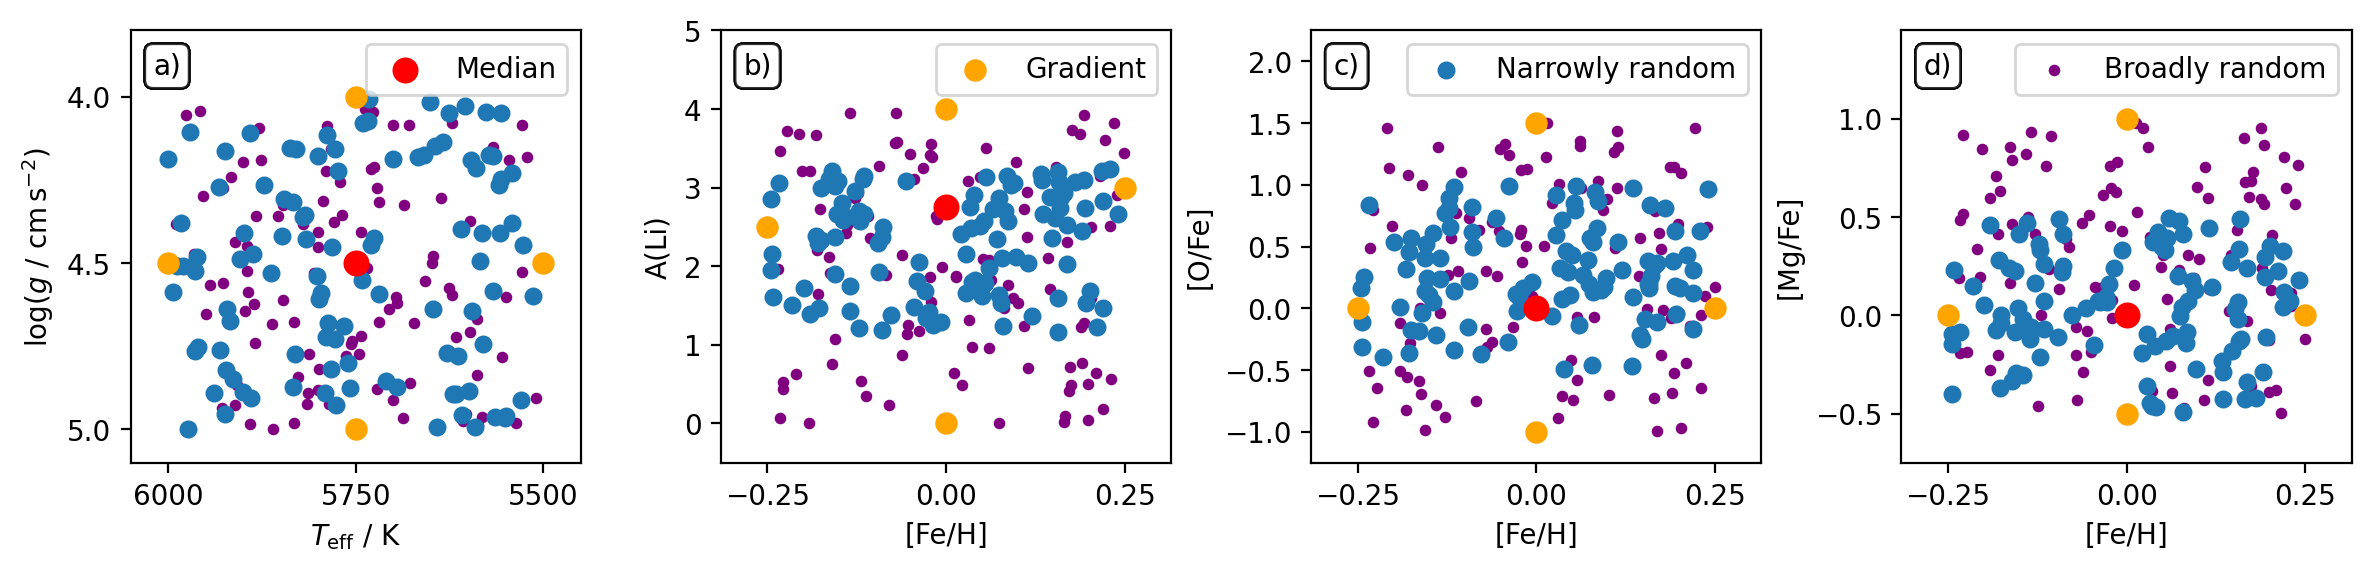
\includegraphics[width=\textwidth]{figures/example_3d_bin_sample.png}
 \caption{\textbf{Coverage of stellar parameters and abundances for one of the 3D bins.} Shown is the example of the solar 3D bin ($T_\mathrm{eff}~/~\mathrm{K} = 5750$, $\log (g~/~\mathrm{cm\,s^{-2}}) = 4.5$, $\mathrm{[Fe/H]}~/~\mathrm{dex} = 0.0$). \textbf{Panel a):} \Teff and \logg, \textbf{Panel b):} [Fe/H] vs. [Li/Fe], \textbf{Panel c):} [Fe/H] vs. [O/Fe], \textbf{Panel d):} [Fe/H] vs. [Mg/Fe]. While \Teff, \logg, and \feh are sampled randomly within the 3D bin, the abundances are sampled both narrowly (blue) and broadly (purple) within limits as described in the text. Red point indicate the median spectrum and orange points the adjusted spectra to test the gradient change of spectra with individual label.}
 \label{fig:example_3d_bin_sample}
\end{figure*}

To achieve a self-consistent grid of synthetic spectra, we compute significantly over-sampled synthetic spectra at 10- times higher then the typical GALAH resolution with \sme.

We select small parts, that is 3D bins of the parameter space of \Teff, \logg, and \feh. For each of these parameters, we loop through the \marcs grid and compute randomly selected spectra within $\pm 1$ grid points in \Teff (with either $\pm 250$ or $\pm 100\K$), \logg ($\pm 0.5\dex$), and \feh ($\pm 1.0$, $\pm 0.5$ or $\pm 0.25\dex $).

We explain the sampling of parameters and abundances in an exemplary way for the 3D bin centred on $T_\text{eff} = 5750\pm250\K$, $\log g = 4.5\pm0.5\dex$ and $\mathrm{[Fe/H]} = 0.0\pm0.25\dex$ (see blue box in Fig.~\ref{fig:teff_logg_grid_coverage}).

For each synthetic spectrum to be computed within this 3D bin, the stellar parameters (\Teff, \logg, \feh, \vmic) and elemental abundances [X/Fe] of all 30 elements are randomly sampled within reasonable limits (see Eqs.~\ref{eq:sampling_teff}-\ref{eq:sampling_xfe}) and fed into \sme to create self-consistent synthetic spectra over the full wavelength range for \marcs atmospheres:
\begin{align} 
    T_\text{eff}~/~\K &\in {5500..5750..6000} \\ \label{eq:sampling_teff}
    \log g~/~\dex &\in {4.0..4.5..5.0} \\
    \mathrm{[Fe/H]}~/~\dex &\in {-0.25..0.0..0.25} \\
    v_\text{mic}~/~\kms &\in Eq.~\ref{eq:vmic_initial} \\
    v \sin i~/~\kms &= 0\text{, but see Eq.~\ref{eq:vsini}} \\
    \mathrm{A(Li)} &\in \begin{cases} {1.05..2.75..3.26} \\ {0.00..4.00} \end{cases} \\
    \begin{array}{l}
    \mathrm{[X/Fe]~for~C,~N,~O, and}\\
    \mathrm{Y,~Ba,~La,~Ce,~Nd}
    \end{array}
    &\in \begin{cases} {-0.5..0.0..1.0} \\ {-1.0..1.5}  \end{cases} \\
    \mathrm{[X/Fe]~for~Mg,~Si,~Ti} &\in \begin{cases} {-0.5..0.0..0.5} \\ {-0.5..1.0}  \end{cases} \\
    \mathrm{[X/Fe]~for~all~other~elements} &\in \begin{cases} {-0.5..0.0..0.5} \\ {-1.0..1.0} \label{eq:sampling_xfe} \end{cases}
\end{align}

% \SB{Write equations for vmic from DR3 \citep{Buder2021} and \citet{DutraFerreira2016} as well as the requirement of at least 0.5 for the uniform sampling.}

\begin{figure}[hbt!]
 \centering
 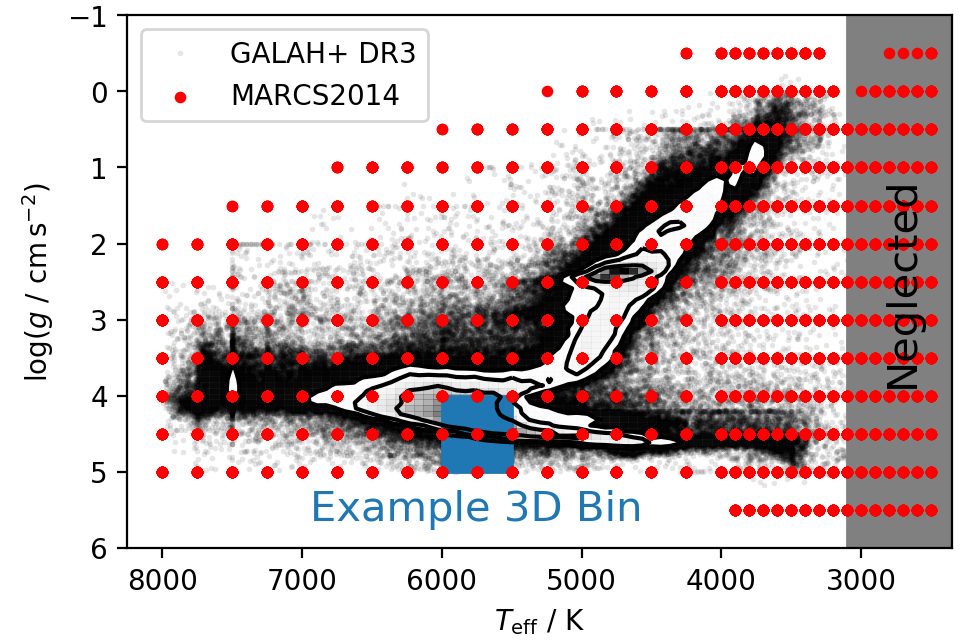
\includegraphics[width=\textwidth]{figures/teff_logg_grid_coverage.png}
 \caption{Coverage in \Teff and \logg of MARCS2014 grid (red) and GALAH DR3 (black, including density countour). Shown is also an example of one of the 3D bins used to create models with \TheCannon. MARCS grid points \Teff$ < 3100\K$ or \feh$<-3\dex$ are neglected throughout GALAH DR4.}
 \label{fig:teff_logg_grid_coverage}
\end{figure}

For each spectrum, we first run a test on all available lines in the GALAH linelist, which is adapted from \citet{Heiter2021} and includes small changes to correct wrong $\log gf$ values for few lines within the GALAH wavelength range. We keep all atomic lines for the final synthesis and restrict the molecular lines to those with \textsc{sme}.depth above 0.001.

Spectra are computed at a resolution of $R = 300,000$ on a fine wavelength grid with 60,819 pixels spread over the extended wavelengths $4675.1- 4949.9$, $5624.1-5900.9$, $6424.1-6775.9$, and $7549.1-7925.9 \Angstroem$. We note that these extend significantly beyond the actual GALAH wavelength range.

We use 1D \marcs atmospheres from the \marcs grid \citep[][version 2014]{Gustafsson2008}, and interpolate them for combinations of \Teff, \logg, and \feh. We use grids of non-LTE departure coefficients by \citet{Amarsi2020} for H, Li, C, N, O, Na, Mg, Al, Si, K, Ca, Mn, and Ba. For all, except C, we use grids that include background scattering.

To be able to test that the flux-label correlations found by our subsequent polynomial interpolation are limited to reasonable wavelength ranges, we also calculate one spectrum that is exactly in the middle of the parameter range and additional spectra, where we increase the value of one label at a time (e.g. increase [O/Fe] by $1\dex$) to test the response in the synthetic spectrum.

To save computational costs, we compute synthetic spectra with no rotational or macroturbulence broadening ($v_\text{mac} = v\sin i = 0\kms$), but save the model continuum flux (\texttt{sme.cmod}) and the specific intensities (\texttt{sme.sint}) as a function of the equal-area midpoints of each equal-area annulus $\mu$ (see Fig.~\ref{fig:sme_mu_output}).

\begin{figure*}[hbt!]
 \centering
 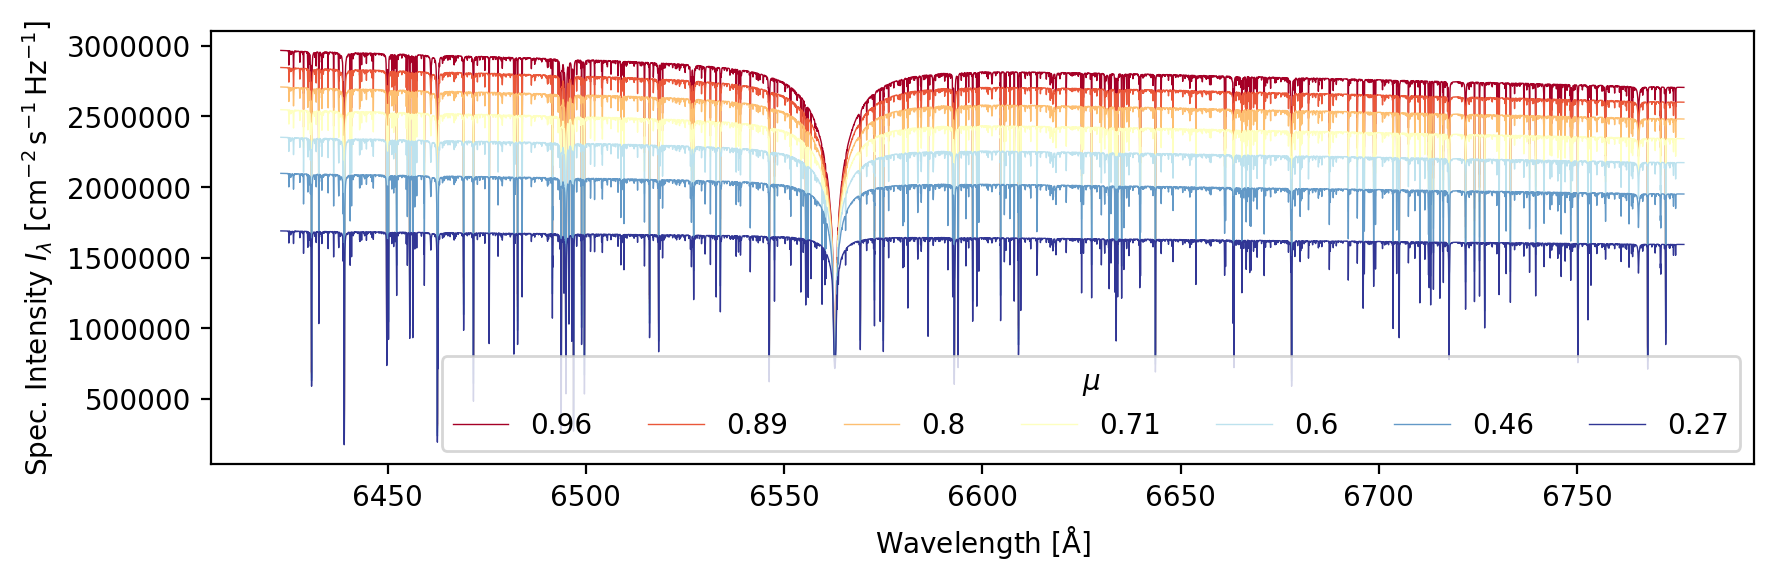
\includegraphics[width=\textwidth]{figures/solar_twin_specific_intensity.png}
 \caption{Example output of \sme for a solar spectrum in HERMES CCD3 (around the Balmer $\mathrm{H}_\alpha$ line). Shown are the the specific intensities (\texttt{sme.sint}) as a function of the equal-area midpoints of each equal-area annulus $\mu$.}
 \label{fig:sme_mu_output}
\end{figure*}

Our synthetic grid explicitly includes C and N abundances. C was previously included in the analysis of GALAH DR3, but limited to the atomic C line. The analysis thus neglected the molecular absorption features of $\mathrm{C_2}$ and CN at the beginning of CCD1 and end of CCD4, respectively. With the new self-consistent grid, we can however include these features, as they hold valuable information for both C and N, as well as several other features through the molecular equilibrium in stars \citep[see e.g.][]{Ting2018}.

In this step, synthetic spectra are calculated for different angles $\mu$ between the outward normal and the line of sight angles and assuming $v \sin i = 0\kms$. 

Once the synthetic spectra are calculated for different angles $\mu$ between the outward normal and the line of sight angles with $v \sin i = 0\kms$, we apply the broadening of spectra due to rotation (\vsini) and sample each of the synthetic spectra over a range of
\begin{align} \label{eq:vsini}
    v \sin i~/~\kms \in \{ 1.5, 3, 6, 9, 12, 18, 24^\star, 36^{\star \star}\}.
\end{align}
% The decision for these values was made based on the distribution of \vsini ($7.2_{-1.6}^{4.9}\kms$ with 90\% between 4.7 and $29.0\kms$) in GALAH+ DR3 \citep{Buder2021} and comparison with the grid values used by APOGEE DR16 \citep{Joensson2020}.

For bins with \Teff$\geq 5000\,\mathrm{K}$, we also include $v \sin i = 24 \kms$ and for those with \Teff$\geq 6000\,\mathrm{K}$ we also include $v \sin i = 36 \kms$. 

In this post-processing steps, we then integrate the flux over these angles and simultaneously broadening the spectra with the different rotational velocities (Eq.~\ref{eq:vsini}). For this we use code from the python-implementation \textsc{PySME} \citep{Wehrhahn2021} of \textsc{SME} \citep{Piskunov2017}.

%%%%%%%%%%%%%%%%%%%%%%%%%%%%%%%%%%%%%%%%%%%%%%%%%%%%%%%%%%%%%%%%%%%%%%%%%
\subsection{Interpolating synthetic spectra with neural networks} \label{sec:interpolating_synthetic_spectra_with_neural_networks}
%%%%%%%%%%%%%%%%%%%%%%%%%%%%%%%%%%%%%%%%%%%%%%%%%%%%%%%%%%%%%%%%%%%%%%%%%

To allow a fast interpolation with new and different stellar labels, we use the method of training descriptive models to connect stellar fluxes at given pixels from a combination of stellar labels. This method is well established in stellar spectroscopy through the successful applications of quadratic models with \textit{The Cannon} \citep[see e.g.][]{Ness2015, Ness2016, Casey2016, Casey2017, Ho2017, Buder2018} as well as neural networks with \textit{The Payne} \citep[see e.g.][]{Ting2019, Xiang2019, Xiang2021}. Because of the needed flexibility\footnote{For a more detailed discussion on the advantages of neural networks for predicting spectra see \citet{Ting2019}.} to predict synthetic spectra with 36 stellar labels for a large parameter space, we are also choosing neural networks to interpolate between our synthetic spectra in this data release.

In particular, we use the neural network architecture and training algorithms of \textit{The Payne} \citep{Ting2019} for our data. We describe the connection of stellar labels $\boldsymbol{\ell}$ and the flux $f$ at each wavelength pixel $\lambda$ via
\begin{equation}
f_\lambda = w \cdot \sigma\bigg( \tilde{w}_\lambda^i \sigma \Big( w^k_{\lambda i} \ell_k + b_{\lambda i} \Big) + \tilde{b} \bigg) + \bar{f}_\lambda,
\label{eq:neural_network_function}
\end{equation}
where $\sigma$ is the Sigmoid function $\sigma (x) = 1/(1 + e^{-x})$ that encapsulates the so called layers of a neural network with $i = 300$ neurons \citep[see ][for more details]{Ting2019}. After optimising a loss function for $10^4$ steps, we consider the network trained with an optimised combination of three sets of weights and biases within the minimum and maximum ranges of each label. The trained networks can then be used with new input labels to quickly create synthetic spectra for the label optimisation.

\SB{Describe the gradient spectra and include 4 examples of Teff, C, N, and Li as shown in Fig.~\ref{fig:gradient_spectrum_5750_4.50_0.00}.}

% The responses for an example 3D bin (again the solar 3D bin), are shown in Figs.~\ref{fig:gradient_spectra_1931_1}-\ref{fig:gradient_spectra_1931_5}, with percentage values listed in Tab.~\ref{tab:cannon_mask_percentage}. Several labels influence almost the entire spectrum. This is not surprising for the stellar parameters \Teff, \logg, \feh, and \vmic. We note, however, also a significant response above 0.001 flux units and 50\% for C, N, O, Mg, and Si. These elements show broad molecular features (like CN in the GALAH wavelength range) or are important electron donors. For N, O, Mg, and Si we even note a strong response for the H Balmer lines. Half of the elements (Li, K, Sc, Cu, Zn, Rb, Sr, Y, Zr, Mo, Ru, Ba, La, Sm, and Eu) are responding solely to their atomic absorption lines and are thus influencing less than 10\% of the spectrum. We find even more minimal changes in the flux below 0.0001, that is below 0.01\% of the normalised flux, for the most extreme cases of labels. 

\begin{figure*}[!ht]
 \centering
 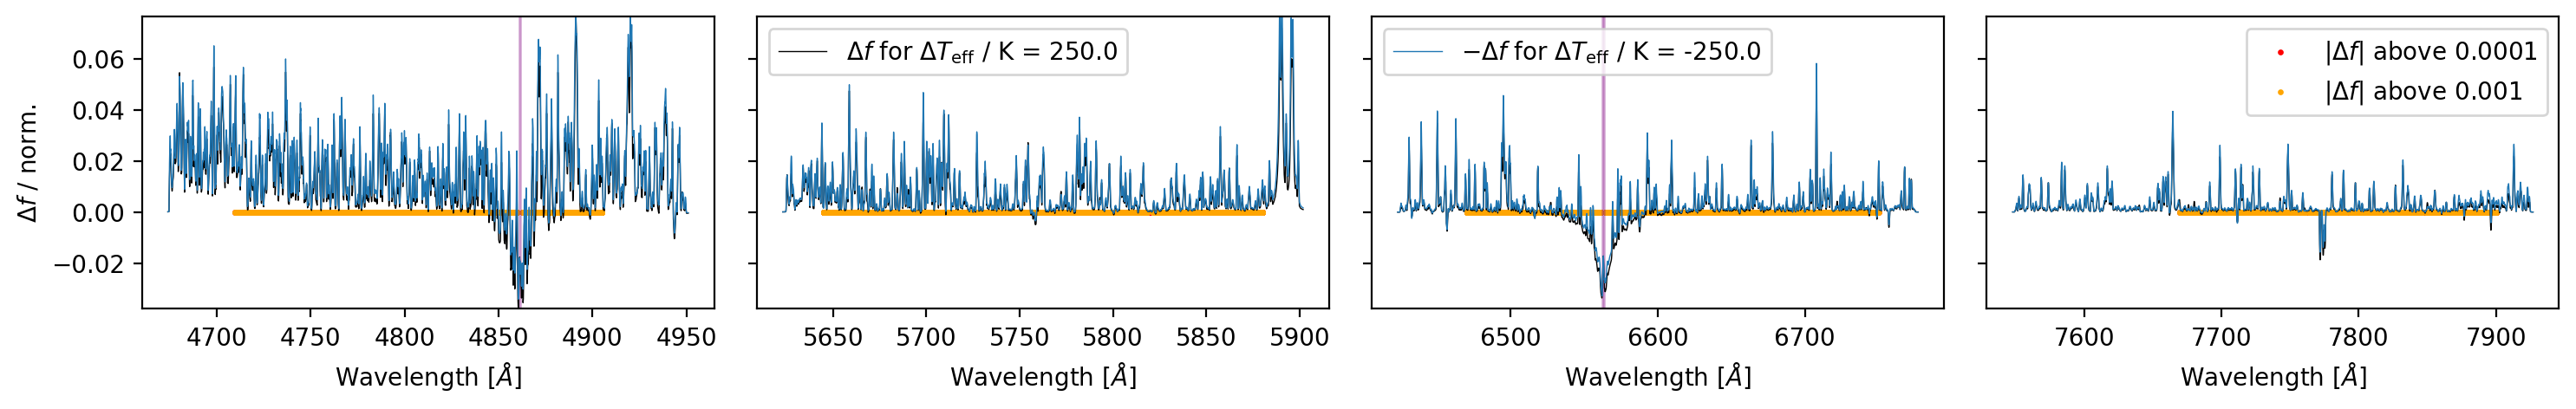
\includegraphics[width=\textwidth]{figures/gradient_spectrum_5750_4.50_0.00_teff.png}
 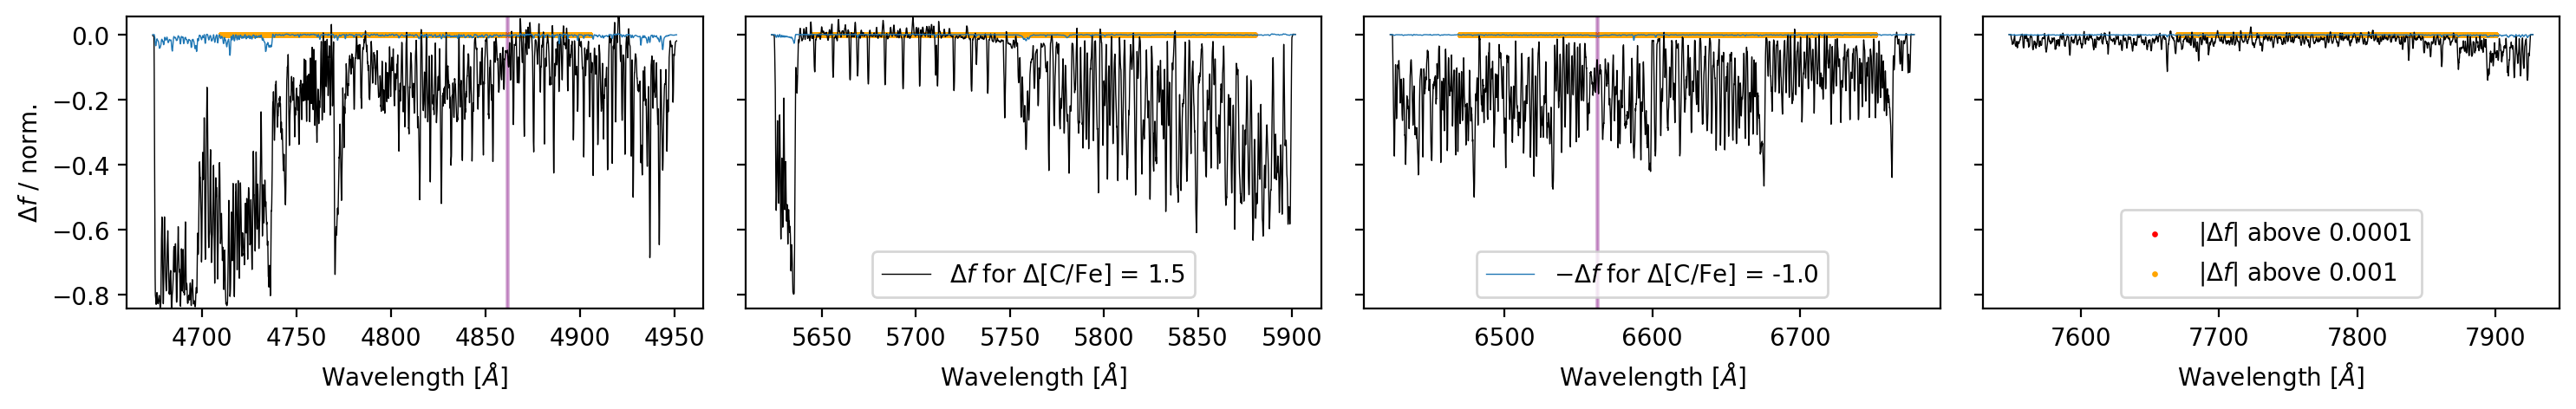
\includegraphics[width=\textwidth]{figures/gradient_spectrum_5750_4.50_0.00_c_fe.png}
 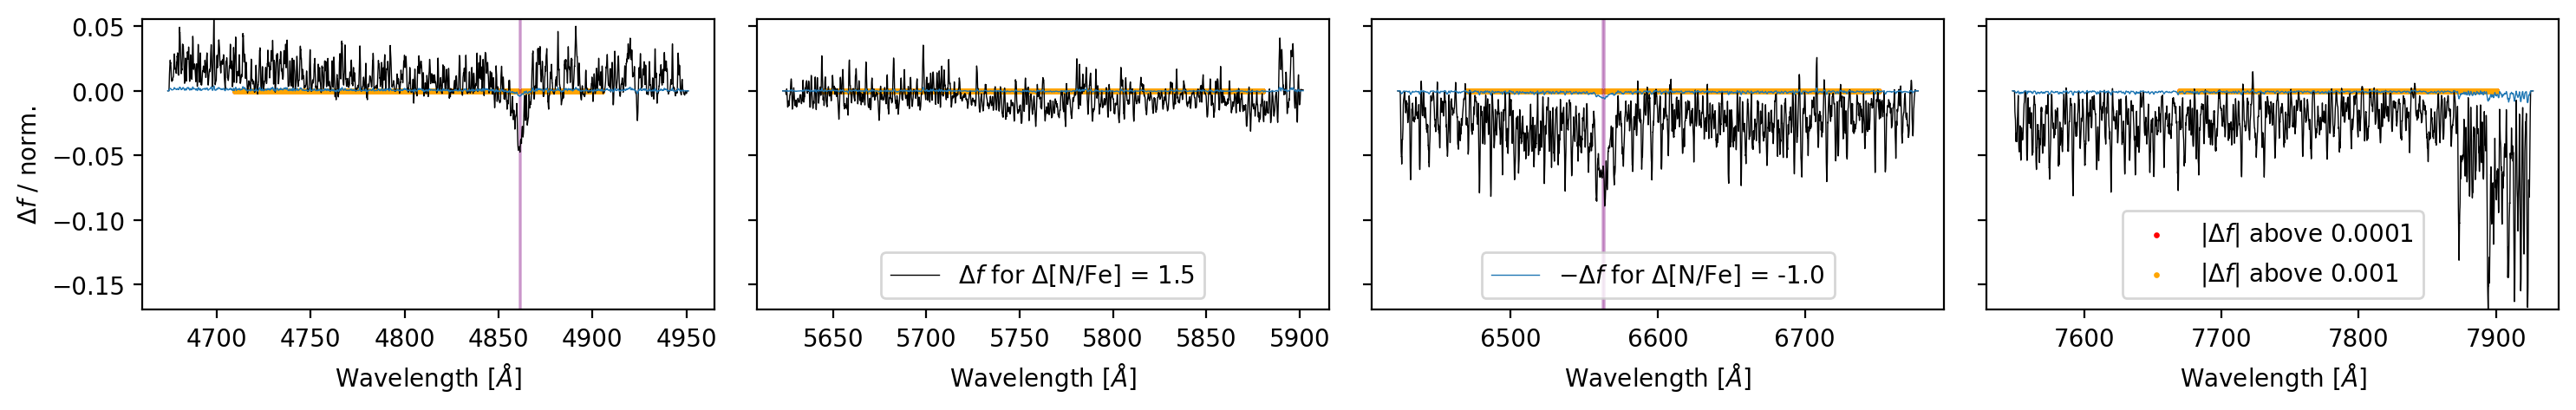
\includegraphics[width=\textwidth]{figures/gradient_spectrum_5750_4.50_0.00_n_fe.png}
 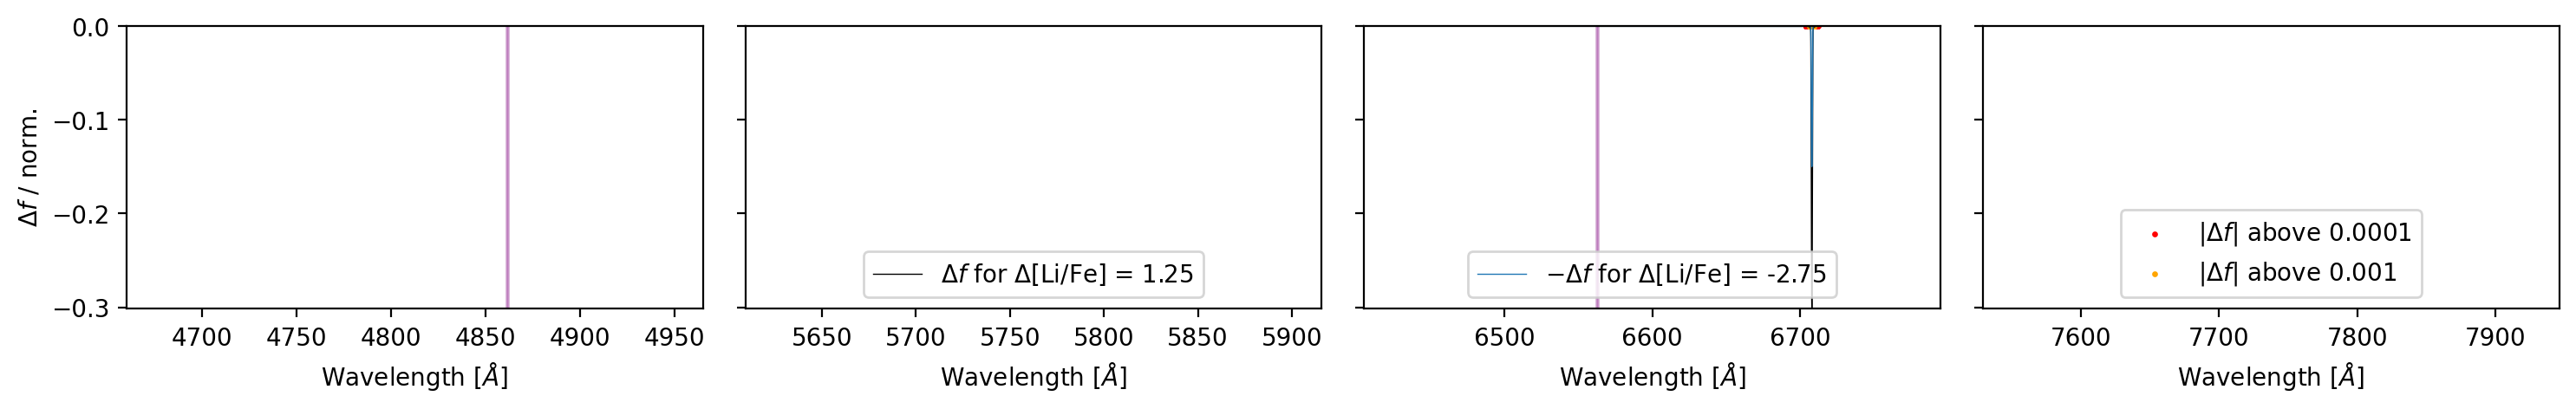
\includegraphics[width=\textwidth]{figures/gradient_spectrum_5750_4.50_0.00_li_fe.png} \caption{\textbf{\sme gradient spectra for the Solar 3D bin (\Teff 5750, \logg 4.5, \feh 0.0, [C/Fe] 0.0, [N/Fe] 0.0, A(Li) 2.75). for the labels \Teff, $\mathrm{[C/Fe]}$, $\mathrm{[N/Fe]}$, and $\mathrm{A(Li)}$.} Shown are differences of the normalised flux when increasing (black) or decreasing (blue) the label values towards the grid limits ($5500/6000\K$, $-1/1.5\dex$, $-1/1.5\dex$, and $0/4\dex$). Purple lines indicate the Balmer line cores. Red and orange dots indicate at which wavelengths normalised fluxes change by more than 0.0001 and 0.001, respectively.
} \label{fig:gradient_spectrum_5750_4.50_0.00}
\end{figure*}

Note that in an earlier version of our grids, we had explored the range of $\mathrm{A(Li)} = -1..5$, which caused sinusoidal shaped of the weak Li line \citep[see also][]{Wang2020}. The synthetic lines stayed in the expected Gaussian-like shape for all our test cases, when limiting the range of $\mathrm{A(Li)}$ to a more reasonable $0..4$.

%%%%%%%%%%%%%%%%%%%%%%%%%%%%%%%%%%%%%%%%%%%%%%%%%%%%%%%%%%%%%%%%%%%%%%%%%
\subsection{Comparison of synthetic spectra to observations}
\label{sec:comparison_synthetic_spectra_to_observations}
%%%%%%%%%%%%%%%%%%%%%%%%%%%%%%%%%%%%%%%%%%%%%%%%%%%%%%%%%%%%%%%%%%%%%%%%%

The major aim of our spectroscopic analysis is to predict the best set of stellar labels by minimising the uncertainty-weighted difference of observed and synthetic spectra. In this section, we describe several important steps to enable the pixel-level comparison of the higher resolution, oversampled synthetic spectra created with the neural networks from Sec.~\ref{sec:interpolating_synthetic_spectra_with_neural_networks} and the observational data at actually measured resolution and sampling (presented in Sec.~\ref{sec:spectroscopic_data_from_galah_observations}).

\subsubsection{Downgrading of synthetic spectrum to observed resolution}

Because dedicated line-spread-function measurements are available for every spectrum (see Sec.~\ref{sec:major_changes_to_previous_data_releases}), we use this information to downgrade our synthetic spectra to the measured resolution of each observations.

We then interpolate the over-sampled synthetic spectrum onto the observed wavelength.

\subsubsection{Re-normalisation of observed spectrum}

Measurements of the GALAH flux and flux uncertainty are reported in counts by the reduction pipeline. To compare with our synthetic spectra, which are normalised to the continuum, we fit an outlier-robust polynomial function to the ratio of observed and synthetic spectrum and re-normalise our observed spectra and their uncertainties via this normalisation function.

This specific approach is similar to the internal routine of \textsc{SME} \citep{Piskunov2017} and has the important advantage, that no continuum points have to be defined. This is advantageous, because we try to cover the full parameter range of FGKM stars for which positions of continuum points -- corresponding to 1 on a (pseudo-)continuum-normalised spectrum -- differ significantly or for which continuum points may not even be present (as is the case for M stars).

% We make two additional adjustments to the reduced spectra, which come in the form of counts and uncertainty per wavelength, $f_\lambda$ and $\sigma_{f,\lambda}$.

% As we compare the observation to model spectra, we do not have to restrict ourselves to an a priory normalisation, but can take into account the residual information on the continuum in parts of the spectra. For each model spectrum that we compare to, we therefore perform a normalisation by fitting a Chebyshev polynomial with outlier clipping to the ratio of model and observation (see Fig.~\ref{fig:ratio_normalisation}). This allows us to both overcome previous shortcomings of the synthetic analysis in GALAH+ DR3 \citep{Buder2021}, which had to be restricted to small wavelength segments and assumed a linear relation for those. Our new approach allows us to properly assess the structure of deep and steep molecular features for cool stars, which dominate spectra of cool stars and carry significant information on \Teff as well as \vrad.

% \begin{figure*}[hbt!]
%  \centering
%  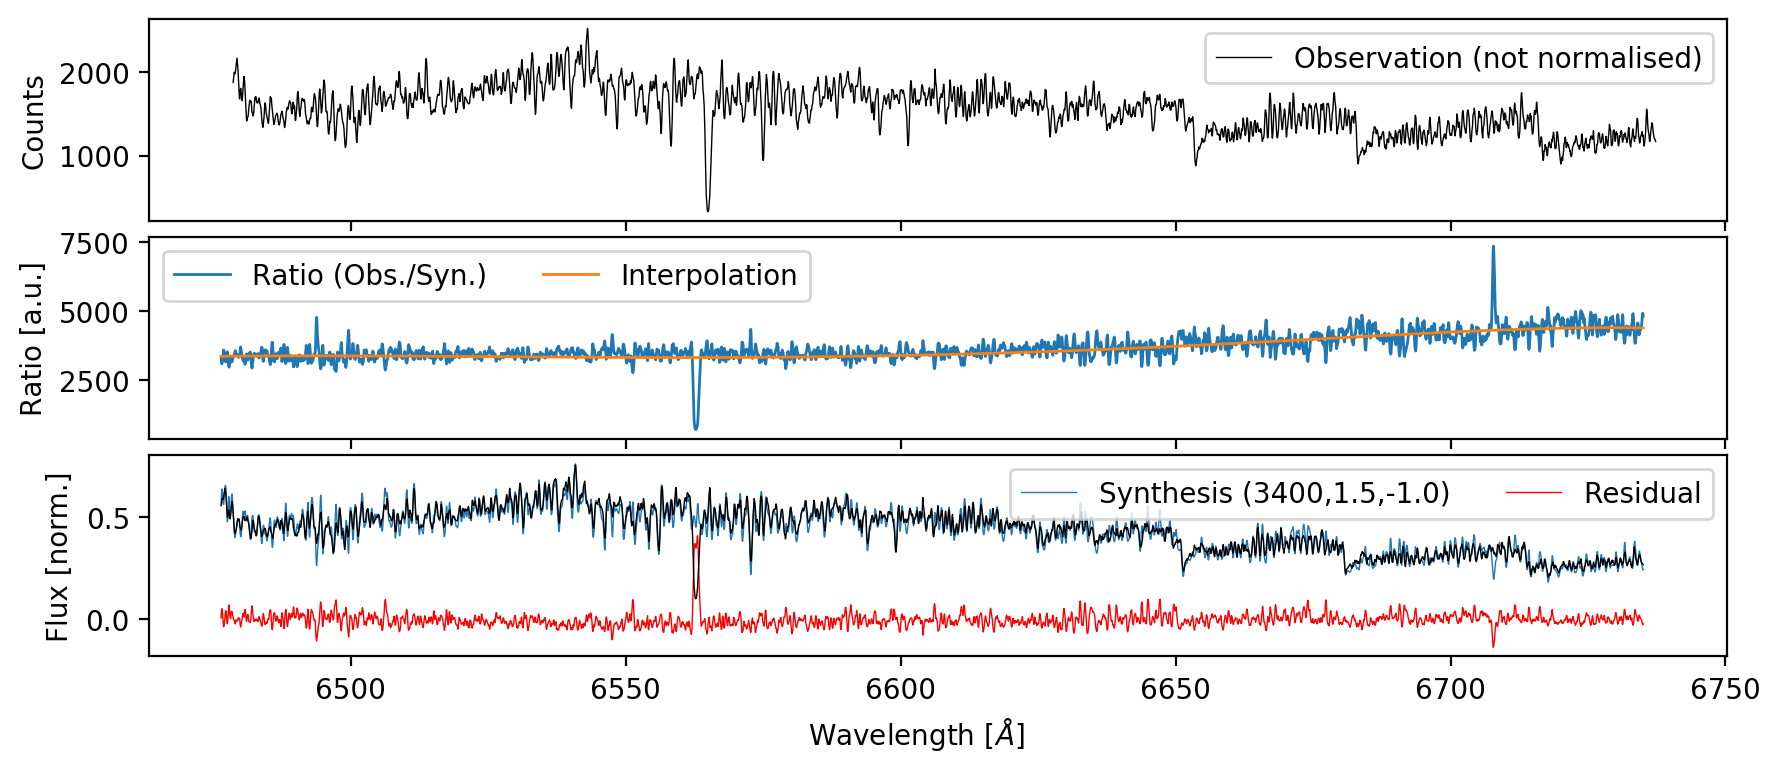
\includegraphics[width=\textwidth]{figures/Nuisance_example.png}
%  \caption{
%  \textbf{Example of normalisation for GALAH DR4 for a model spectrum that is selected during the label optimisation.}
%  \textbf{Panel (a):} Observed spectrum (counts) of star 2MASS XYZ.
%  \textbf{Panel (b):} Ratio (blue) of observed spectrum and model spectrum as well as Chebychev polynomial fit (orange).
%  \textbf{Panel (c):} Normalised observed spectrum (black) compared to the model spectrum (blue). Residuals (red) can then be used as input for the likelihood function.
%  }
%  \label{fig:ratio_normalisation}
% \end{figure*}

% For each CCD, the reduction has found the most suitable wavelength solution, linking pixels with actual wavelengths, based on the ThXe arc lines. In GALAH DR3 \citep{Buder2021}, we have found several issues for spectra, where not enough ThXe lines could be used to constrain the wavelength solution. Improvements have been made for the new reduction version to improve the number of useful ThXe lines. Two additional pieces of information are, however, unused by the reduction pipeline, namely (i) the telluric lines\footnote{\SB{Check with Janez if that is actually still true!}} that are present throughout GALAH spectra and (ii) the absorption lines of the stellar spectra. Both hold valuable information, as their position (in rest wavelength) is known very well.

% The reduction is providing spectra and other parameters in an array of $n$ pixels, that is linked to wavelengths $\lambda_n$ through a linear function
% \begin{align} \label{eq:wavelength_solution}
%     \lambda (n) = \lambda_0 + n \cdot \Delta_\lambda.
% \end{align}
% In particular, for each CCD, the pipeline reports $\lambda_0$ as \texttt{cdelt} and $\Delta_\lambda$ as \texttt{CRVAl}.\footnote{\SB{Can we take into account uncertainties on these values through the pipeline? e.g. rms?}}
% Because we can directly compare to model spectra with a perfect wavelength solution, we therefore allow these eight values (two for each of the four CCDs) to be fitted by our analysis pipeline.

% \SB{Could this be degenarate with \vrad. Could be solved by (i) keeping one CCD fixed or (ii) adding a fit to the telluric lines as well, because we know their dependence on wavelength!}



% \subsubsection{Selecting the best model for the labels at hand}

% For each combination of \TLF, we finding \TheCannon's nearest neighbor model via .

% \SB{Describe here the tests we do to make sure this actually provides a smooth transition between the different labels. Tests of the Cannon models show, that they can reproduce the spectra and their labels within for example $1\K$ \Teff, $0.01\dex$ \logg, and $0.01\dex$ \feh for the grid edges. But more thorough testing is needed.}

% \SB{Also keep in mind the issues found for \TheCannon with only 2 models applied to RAVE \citep{Casey2017}.}

%%%%%%%%%%%%%%%%%%%%%%%%%%%%%%%%%%%%%%%%%%%%%%%%%%%%%%%%%%%%%%%%%%%%%%%%%
\subsection{Stellar label optimisation}
\label{sec:stellar_label_optimissation}
%%%%%%%%%%%%%%%%%%%%%%%%%%%%%%%%%%%%%%%%%%%%%%%%%%%%%%%%%%%%%%%%%%%%%%%%%

\subsubsection{Stellar label estimation assuming single star}
\label{sec:stellar_label_estimation_assuming_single_star}

\paragraph{Workflow of the optimisation}

In up to four major loops, we optimise the radial velocities and all other stellar labels and report a) their values, b) their co-variances, c) the best fit synthetic and re-normalised spectra along with their uncertainties and masks that indicate which pixels were used in the final optimisation.

Starting from the initial values, a first synthetic spectrum is computed and compared with the observation in order to assess the initial radial velocity. This is done by applying the \textsc{scipy.signal.find\_peaks} algorithm on a the residuals\footnote{We use the inverse of the residuals that were normalised with the smallest residual values.} of non-shifted observed and synthetic spectra, when the latter is shifted by $v_\text{rad} = -1000..(2)..1000\kms$ (see Fig.~\ref{fig:181221003101356_single_fit_rv}a). If no peak is found, the initial \vrad value is used hereafter. If more than one peak is found (see Fig.~\ref{fig:181221003101356_single_fit_rv} with \Gaia DR3 agreeing with the systemic radial velocity), the two strongest peaks are reported and trigger a stellar label estimation assuming binary star (Sec.~\ref{sec:stellar_label_estimation_assuming_binary_star}. For the purpose of the single star analysis, a narrower search is conducted around the highest peak with a \vrad shift of $-20.00..(0.04)..20.00\kms$ around said peak by fitting a Gaussian function to the inverse of the residuals that were normalised with the smallest residual values (see Fig.~\ref{fig:181221003101356_single_fit_rv}c). The mean of this fit and its uncertainty are reported by the pipeline.

\begin{figure}[hbt!]
 \centering
 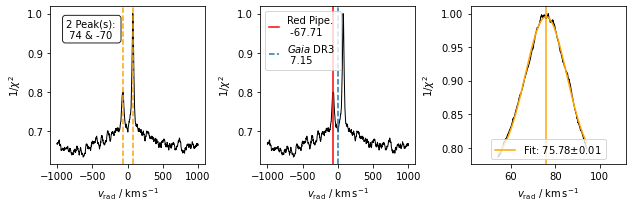
\includegraphics[width=\textwidth]{figures/181221003101356_single_fit_rv.png}
 \caption{\textbf{Output of the radial velocity fitting module.} \textbf{Panel a)} shows the initial broad search on a \vrad array of $-1000..(2)..1000\kms$. In the case of 2MASS J06084657-7815235, two peaks (yellow, dashed) are visible for this line-splitting spectroscopic binary. \textbf{Panel b)} shows the same plot, but overlaid with the GALAH DR4 reduction pipeline (red) and \Gaia DR3 (blue, dashed) estimates. \textbf{Panel c)} shows the narrow window of $-20.00..(0.04)..20.00\kms$ around the highest peak and the Gaussian fit (yellow) to it.}
 \label{fig:181221003101356_single_fit_rv}
\end{figure}

The centerpiece of our optimisation is the \textsc{scipy.optimise.curve\_fit} function, which we call with counts and uncertainties (\texttt{absolute\_sigma = True}) as input to estimate the labels via the least squares optimisation within less than $10^4$ iterations and a desired relative error (\texttt{xtol}) below 0.0001.

For the each optimisation loop, a new, best-fit 3D bin and neural network is identified via a grid search in the \TLF dimensions with \textsc{sklearn.cKDtree}. If the stellar labels that are being fitted have changed (for example if an element is deemed not detectable for the new 3D bin), the label and its value is either deleted or initialised with $\mathrm{[X/Fe]} = 0$.

While the optimisation has not converged (the final parameters \TLF are not within the current 3D bin), the optimisation is repeated, starting with the previous best-fit parameters as starting guesses.

\paragraph{Initial and intermediate label values}

Initial values of all stellar labels are needed for creating a first synthetic spectrum. For \vrad, \Teff, \logg, and \vsini we use a combination of sources, namely the GALAH DR4 reduction pipeline, GALAH DR3 \citep{Buder2021}, $\Gaia$ DR3 \citep{Brown2021}, and 2MASS \citep{Skrutskie2006}. In selected cases, we adjust the starting parameters towards reasonable limits. Below we briefly describe the general approach to finding initial values, but refer to the \href{https://github.com/svenbuder/GALAH_DR4/blob/main/spectrum_analysis/galah_dr4_initial_parameters.ipynb}{online repository} for the detailed implementation. 

Based on the chosen \Teff and \logg, we then apply calculate an initial value for \vmic within limits of $0.5$ to $4.0\kms$ based on Eq.~\ref{eq:vmic_initial} for $T_\text{eff}^\prime = T_\text{eff} - 5500\,\mathrm{K}$ as well as $\log g^\prime = \log g - 4.0$:
\begin{align} 
v_\text{mic} = \begin{array}{l}
1.198 + 3.16 \cdot 10^{-4} \cdot T_\text{eff}^\prime - 0.253 \cdot \log g^\prime \\ - 2.86\cdot 10^{-4} \cdot T_\text{eff}^\prime \cdot \log g^\prime + 0.165 \cdot \log g^\prime
\end{array} \label{eq:vmic_initial}
\end{align}
This relation is shifted by $+0.2\kms$ from the originally reported relation by \citet{DutraFerreira2016} based on 3D model atmospheres.

Based on the value of \feh we apply an offset to the $\mathrm{\alpha}$-elements O, Mg, Si, Ca, and Ti within our wavelength range. The initial value is 0.4 for $\mathrm{[Fe/H]} < -1$, 0.0 for $\mathrm{[Fe/H]} > 0$, and $-0.4\cdot \mathrm{[Fe/H]}$ for $-1 \leq \mathrm{[Fe/H]} \leq 0$. All other abundances are initialised at $\mathrm{[Fe/H]} = 0$.

\SB{Describe more of the special cases and when what is used in combination with the reference to Fig.~\ref{fig:initial_parameters}.}
% https://github.com/svenbuder/GALAH_DR4/blob/main/spectrum_analysis/galah_dr4_initial_parameters.ipynb

\paragraph{Which labels are optimised?}

% This paragraph is based on the combination of 
% spectrum_interpolation/galah_dr4_grid_interpolation_recommend_labels.ipynb
% and
% spectrum_analysis/galah_dr4_spectrum_analysis_single.ipynb

As part of the synthetic grid computations, we have perturbed each label individually to our chosen maximum and minimum ranges (see Sec.~\ref{subsubsec:spectrum_grid}). This allows us to also judge which stellar labels to fit for each given star. We choose to fit a stellar label, if either of the two cases applies to said label for the GALAH wavelength range when neglecting the cores of the Balmer lines: Does the spectrum between minimum and maximum label value at any pixel change more than a certain threshold (0.07 of the normalised spectrum)? Does the spectrum between minimum and maximum label value change by more than 0.005 of the normalised spectrum for at least 25\% of the spectrum? While the first case is constructed for atomic lines, such as \ion{Li}{i} 6708, the second case is addressing in particular molecular lines like the $\mathrm{C_2}$ and $\mathrm{CN}$ lines. For spectra that are missing the infrared arm (CCD4) we exclude the otherwise possibly fit labels for N, O, L, and Rb.

Initial tests of the pipeline have revealed that in cases where the initial parameter guesses are deviating significantly from the final ones, several elemental abundance estimates were shifted towards their boundaries, leading to a masking of their elemental abundances lines by the masking module (Sec.~\ref{sec:masking_of_unreliable_wavelength_regions}) at the beginning of each optimisation loop. To minimise this effect, we therefore shift the interim abundance values towards the narrow label boundaries. In practise, we this limit the initial and interim abundances to 1.05..3.26 for A(Li), $\mathrm{[X/Fe]} = -0.5..1.0$ for C, N, O, Y, Ba, La, Ce, and Nd, and $\mathrm{[X/Fe]} = -0.5..0.5$ for all other elements before optimising them again. For warm and hot stars ($T_\text{eff} > 6000\K$), this effect was seen to effect multiple abundances, such that we needed to implement a zeroing of all abundances (except Lithium) for stars above $6000\K$, which would on average be expected to be young and have a solar-like composition.

\SB{Mention issues with \vsini going unreasonably high for some giants (>10kms), causing [C/Fe] to go high as well, with chi2/gradient descent seemingly not being able to control this process. This issue was also realised after GALAH DR3 with several of the coolest giants. To guide the pipeline, we therefore implement a hard upper limit of the initial values of each optimisation of $v \sin i = 8km/s$ for giant stars with $T_\text{eff} < 5000$, $\log g < 3$, $v \sin i > 10km/s$. If [C/Fe] was a fitted label for these stars, we also reset it to 0. OR: We adjust the initial values at the beginning?}

\subsubsection{Stellar label estimation assuming binary star} \label{sec:stellar_label_estimation_assuming_binary_star}

% spectrum_analysis/galah_dr4_spectrum_analysis_binary.ipynb

motivated by the extensive study of GALAH binary star spectra by \citet{Traven2020}.

In our strictly spectroscopic implementation, we only use the stellar GALAH spectra and the two radial velocity peaks identified in the radial velocity optimisation step (see Fig.~\ref{fig:181221003101356_single_fit_rv}) of the single star analysis (Sec.~\ref{sec:stellar_label_estimation_assuming_single_star}).

Fitting RV1, RV2, Teff1, Teff2, logg1, logg2, FeH, vmic1, vmic2, vsini1, vsini2

\subsubsection{Masking of unreliable wavelength regions} \label{sec:masking_of_unreliable_wavelength_regions}

Not all pixels of the observed or synthetic spectra might prove useful for estimating reliable stellar labels. Observations can include bad pixels/patterns and incorrect corrections (for example of telluric or sky lines). Flux predictions of synthetic spectra are only as good as the input physics (limited for example for specific lines via uncertain oscillator strengths).

% Based on https://github.com/svenbuder/GALAH_DR4/blob/main/spectrum_analysis/galah_dr4_solar_analysis.ipynb
To minimise the influence of inaccurate synthetic pixel predictions, we have compared a 2dF-HERMES observation of the asteroid 4~Vesta and a high-quality  Solar spectrum by \citet{Hinkle2000} with the flux that would be predicted through our pipeline for a star with Solar labels ($T_\text{eff} = 5772\K$, $\log g = 4.438\dex$, $\mathrm{[Fe/H]} = 0.00\dex$, $v_\text{mic} = 1.06\kms$, $v \sin i = 1.6\kms$, $v_\text{mac} = 4.2\kms$ \citep{Prsa2016, Jofre2017}, and $\mathrm{[X/Fe]} = 0.00\dex$ for the default Solar abundance pattern for \marcs by \citet{Grevesse2007}).

\begin{figure*}[hbt!]
 \centering  
 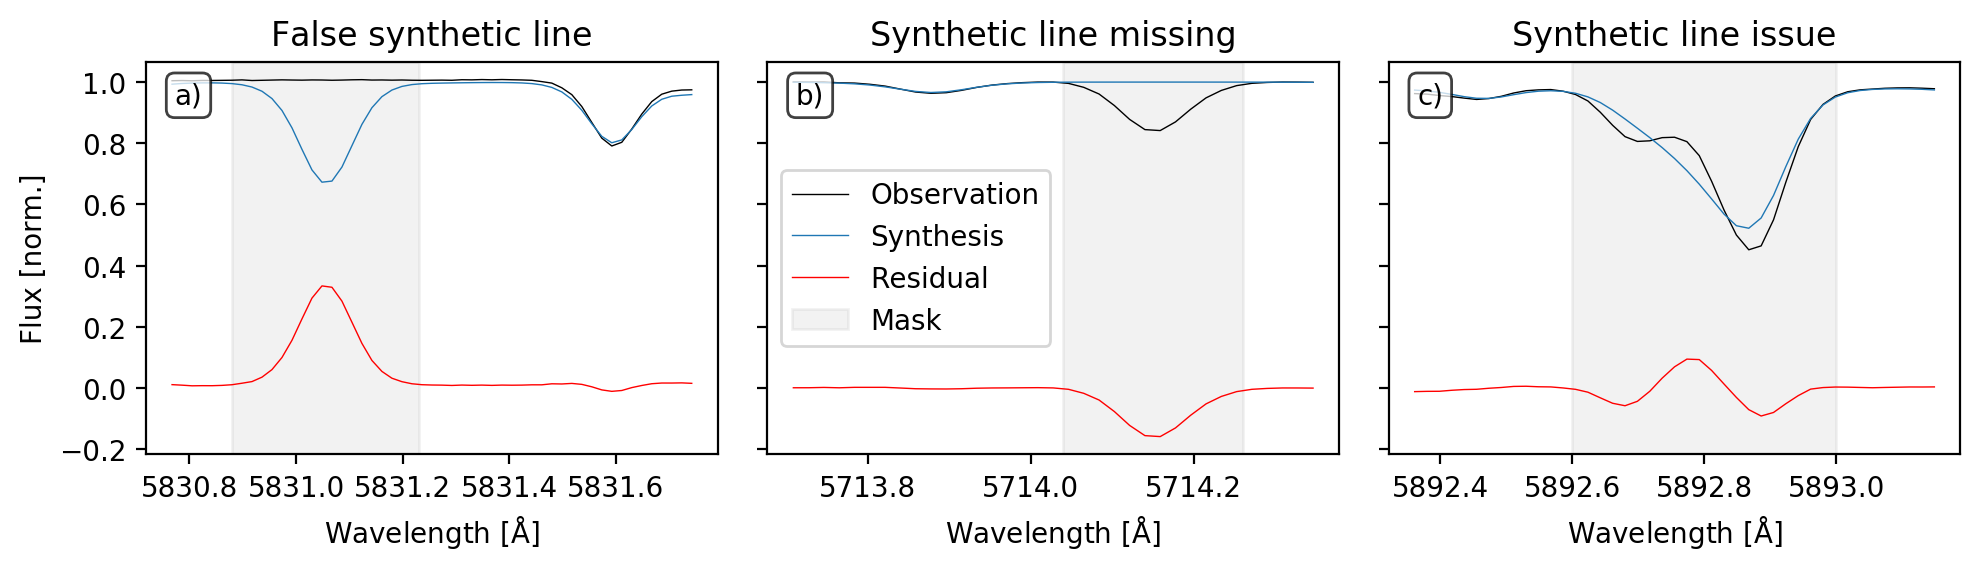
\includegraphics[width=\textwidth]{figures/example_masking_sun.png}
\caption{\textbf{Examples of masks applied to unreliable pixels for the spectrum fitting, that is the minimisation of residuals (red) between observation (black) and synthesis (blue).} \textbf{Panel a)} showing a strong synthetic line, where no line is observed in the Sun. \textbf{Panel b)} showing an observed line without any line being synthesised. \textbf{Panel c)} showing significant disagreement between the two observed lines and the synthesis.} \label{fig:example_masking_sun}
\end{figure*}

We have identified all lines that showed differences of the normalised flux of more than $0.1$, lines where either a synthetic line or an observed one was completely missing, or lines that were significantly misaligned. Examples of this \href{https://github.com/svenbuder/GALAH_DR4/blob/main/spectrum_analysis/spectrum_masks/solar_spectrum_mask.fits}{list} of masks are shown in Fig.~\ref{fig:example_masking_sun}. To avoid the influence of bad spectrum regions with an observational origin, we mask pixels where the synthetic and re-normalised observed spectrum differ by more than $5\sigma$ or a flux of 0.3 (0.4 before the initial optimisation). To avoid the masking of lines that are vital for our spectroscopic analysis, we have created a \href{https://github.com/svenbuder/GALAH_DR4/blob/main/spectrum_analysis/spectrum_masks/vital_lines.fits}{list} with segments of such lines that is mainly based on the previous element masks from GALAH DR3 \citep{Buder2021}. The final mask of pixels to use for the optimisation then includes all vital line regions and those wavelengths that are not unreliable in the synthesis show a too strong disagreement between observation and synthesis.

We further indirectly take into account the currently less constrained molecular data for cool stars in optical spectra, in particular towards the blue (REF from A. Rains). For presumably cool stars (with initial $T_\text{eff} < 4100\,\mathrm{K}$), we therefore double the observational uncertainty of the blue arm.

%%%%%%%%%%%%%%%%%%%%%%%%%%%%%%%%%%%%%%%%%%%%%%%%%%%%%%%%%%%%%%%%%%%%%%%%%
\section{ASTROPHYSICAL ANALYSIS}
\label{sec:astrophysical_analysis}
%%%%%%%%%%%%%%%%%%%%%%%%%%%%%%%%%%%%%%%%%%%%%%%%%%%%%%%%%%%%%%%%%%%%%%%%%

% Finally, we implement a Bayesian framework to estimate consistent astrophysical parameters: we first only use spectroscopic information to estimate the most likely set of stellar labels (stellar parameters and abundances) to describe our data. In a second iteration, we also employ non-spectroscopic information as prior information to inform our analysis. We will denote posterior probability functions depending on the available/used observables:
% \begin{align}
%     P_\text{S} \quad &: \quad \text{only spectroscopy assuming single star,} \\
%     P_\text{B} \quad &: \quad \text{only spectroscopy assuming binary star,} %\\
%     % P_\text{SP} \quad &: \quad \text{also photo- and astrometry, and} \\
%     % P_\text{SPA} \quad &: \quad \text{also asteroseismology.}
% \end{align}

% We present the Bayesian framework to compute these functions in Sec.~\ref{subsec:bayes}. The link between these functions and our observables are several physical relations as well as models, most importantly the models that link stellar flux with stellar parameters and abundances. We describe this centerpiece of our spectroscopic analysis in Sec.~\ref{subsec:model_spectra} and how we adjust the observed spectra to best overcome imperfections based in the reduction on-the-fly in Sec.~\ref{subsec:adjustments_observation}. The machinery to find the best set of labels to describe our observables is described in Sec.~\ref{subsec:finding_best_labels}. The post-processing of outcomes on a spectrum-by-spectrum basis is described in Sec.~\ref{sec:post_processing} and the pipeline is validated in Sec.~\ref{sec:validation}.

% \subsection{Bayesian framework} \label{subsec:bayes}

% Previous versions of the GALAH pipelines used strict $\chi^2$ optimisation \citep{Buder2018} or treated non-spectroscopic information as ground-truth for computational reasons \citep{Buder2021}.

% With the new modelling methodology available this data release, we are inspired by the previous works \citep[e.g.][]{Schoenrich2014, BailerJones2015, McMillan2018, Sharma2018} to simultaneously make a statistically more sound use of non-spectroscopic and prior information. 

% We present the observables $\boldsymbol{y}$ and their uncertainties $\sigma_{\boldsymbol{y}}$ of our analysis in Sec.~\ref{subsubsec:observables}. In Sec.~\ref{subsubsec:labels}, we introduce the set of parameters, hereafter called labels $\boldsymbol{l}$ to generate models/predictions $\boldsymbol{y}_m(\boldsymbol{l})$ of the observables. Our analysis applies a simplified Bayesian statement
% \begin{align}
%     P( \boldsymbol{l} \vert \boldsymbol{y},\sigma_ {\boldsymbol{y}}) \propto P (\boldsymbol{y} \vert \boldsymbol{l}, \sigma_{\boldsymbol{y}}) P (\boldsymbol{l}).
% \end{align}
% Note here, that we ignore the normalisation constant $P(\boldsymbol{y}, \sigma_ {\boldsymbol{y}})$. We present our likelihood functions $P (\boldsymbol{y} \vert \boldsymbol{l}, \sigma_ {\boldsymbol{y}})$ in Sec.~\ref{subsubsec:likelihood} and the prior functions $P (\boldsymbol{l})$ in Sec.~\ref{subsubsec:prior}.

% Because we run our pipeline with different sets of observables, we describe the different sets of probability functions $P( \boldsymbol{l} \vert \boldsymbol{y},\sigma_ {\boldsymbol{y}})$ in Sec.~\ref{subsubsec:probability}, which we will sample in order to create probability density functions (pdfs).

% \subsubsection{Observables} \label{subsubsec:observables}

% The industrial revolution in stellar surveys has allowed us to collect a plethora of spectroscpic ($f_\lambda~\pm~\sigma_{f_\lambda}$), photometric ($m_i~\pm~\sigma_{m_i}$), astrometric ($\varpi~\pm~\sigma_\varpi$), asteroseismic ($\nu_\text{max}~\pm~\sigma_{\nu_\text{max}}$ and $\delta_\nu~\pm~\sigma_{\delta_\nu}$)\SB{, and interferometric ($\Theta_\text{LD} \pm \sigma_{\Theta_\text{LD}}$)} measurements of stars. Each contribute ${\boldsymbol{y}_i} \pm \sigma_{\boldsymbol{y}_i}$ to our set of observables ${\boldsymbol{y}} \pm \sigma_{\boldsymbol{y}}$.

% In our case, the GALAH reduction pipeline delivers $f_\lambda~\pm~\sigma_{f_\lambda}$ (see Sec.~(sec:reduction), but throughout our estimation of optimal stellar labels, we perform several adjustments to the data on-the-fly (see Sec.~\ref{subsec:adjustments_observation}).

% We make use of photometric measurements from both the \Gaia mission \citep{Gaia-Collaboration2016}, specifically its eDR3 \citep{Brown2021}, and 2MASS \citep{Skrutskie2006}. The latter provides near infrared magnitudes $m_J$, $m_H$, and $m_{K_\text{S}}$. We use the three \Gaia bandpasses $m_G$, $m_{G_\text{BP}}$, and $m_{G_\text{RP}}$. We correct the $G$ flux and estimate the \Gaia magnitude uncertainties as described by \citet{Riello2021}. We use astrometric information $\varpi~\pm~\sigma_\varpi$ is provided by \Gaia eDR3 \citep{Lindegren2021a} and we apply the zero point correction to these measurements as described by \citep{Lindegren2021b}. Crossmatches to these catalogues are performed with \textsc{ADQL} queries on the \Gaia archive via \textsc{astroquery} by linking catalogue entries through the \texttt{source\_id} via the nearest neighbor matches provided by the \Gaia consortium on the \Gaia archive \citep[see][]{Marrese2017, Marrese2019}

% We further crossmatch with the open cluster catalogue by \citet{CantatGaudin2020}\footnote{\SB{Update on this with \Gaia eDR3 as part of his 2021 paper?}} via \texttt{source\_id} and use their parallax estimates for stars with more than $70\%$ membership probabilities and more precise parallaxes. Similarly, we crossmatch with the globular cluster catalog by \citet{Vasiliev2021} via \texttt{source\_id} and use their parallax estimates for stars with more than $70\%$ membership probabilities and more precise parallaxes for the clusters NGC~104~/ 47~Tuc, NGC~288, NGC~362, NGC~1851, NGC~5139~/ $\omega$Cen, NGC~6362, NGC~6397, and NGC~7099~/ M~30.

% Where available, we further use the asteroseismic parameters $\nu_\text{max}~\pm~\sigma_{\nu_\text{max}}$ and $\delta_\nu~\pm~\sigma_{\delta_\nu}$ by \SB{Zinn et al. (2021)}\footnote{\SB{Check this! What do we do if not all entries have uncertainties?}}.

% \SB{For interferometric information ($\Theta_\text{LD} \pm \sigma_{\Theta_\text{LD}}$), we use a collection by \citet{Karovicova2020}, \citet{Karovicova2018}, and \citet{Heiter2015}, preferring the most recent values for each star.\footnote{\SB{Check this and also point to a catalog for people to trace back which one was used in the end... for each star. Also do not forget to cite the sources within \citet{Heiter2015}!}}}

% \subsubsection{Model parameters (labels)} \label{subsubsec:labels}

% To describe these observables (and their presumably Gaussian uncertainties), we can build models based on a specific set of parameters, hereafter called labels $\boldsymbol{l}$.

% To predict a normalised stellar spectrum with flux $f \pm \sigma_f$, we need labels $\boldsymbol{l}_S$ that describe the photosphere of a star
% \begin{align}
%     \boldsymbol{l}_\text{S} \in \{
%     T_\text{eff}, \log g, \mathrm{[Fe/H]}, \mathrm{[X/Fe]}, v_\mathrm{mic}, v \sin i, v_\text{rad}
%     \}.
% \end{align}

% To describe photometric measurements of stars, typically reported in magnitudes $m_i \pm \sigma_{m_i}$ for filters $i$ with different bandpasses, we need a similar set of labels and information on the distance and extinction to properly scale a model star,
% \begin{align}
%     \boldsymbol{l}_\text{P} \in \{ T_\text{eff}, \log g, \mathrm{[Fe/H]}, \mathrm{[X/Fe]}, D_\varpi, A_V \}.
% \end{align}
% The distance will also allow us to predict measurements of parallaxes $\varpi \pm \sigma_\varpi$.

% To describe the solar-like oscillations within low-mass stars, which can be transcribed to oscillation frequencies $\nu_\text{max} \pm \sigma_{\nu_\text{max}}$ \SB{and $\delta_\nu \pm \sigma_{\delta_\nu}$} via empirical asteroseismic scaling relations, we need \Teff, \logg, and masses,
% \begin{align}
%     \boldsymbol{l}_\text{A} \in \{ T_\text{eff}, \log g, \mathcal{M} \}.
% \end{align}

% Note that to avoid redundancy with labels in $\boldsymbol{l}_\text{S}$ and $\boldsymbol{l}_\text{P}$, we prefer the use of \logg over radius $\mathcal{R}$, which are fundamentally linked via $R = \sqrt{\mathrm{G} \mathcal{M} g^{-1}}$.

% \subsubsection{Likelihood functions} \label{subsubsec:likelihood}

% Assuming that the uncertainties $\sigma_{\boldsymbol{y}_i}$ of our observables $\boldsymbol{x}$ are Gaussian, we can define a likelihood for each individual observable ${\boldsymbol{y}_i}$ with a model prediction $\boldsymbol{y}_{i,m} (\boldsymbol{l})$
% \begin{align}
%     G({\boldsymbol{y}_i}, {\boldsymbol{y}_{i,m}} (\boldsymbol{l}), \sigma_y) = \frac{1}{\sqrt{2\pi} \sigma_{\boldsymbol{y}_i}} \exp \left( -  \frac{\left({\boldsymbol{y}_i} - {\boldsymbol{y}_{i,m}} (\boldsymbol{l})\right)^2}{2 \sigma_{\boldsymbol{y}_i}^2}\right)
% \end{align}
% or in logarithmic form
% \begin{align}
%     \ln G({\boldsymbol{y}_i}, {\boldsymbol{y}_{i,m}} (\boldsymbol{l}), \sigma_{\boldsymbol{y}_i}) = - \frac{1}{2} \left( \ln (2 \pi \sigma_y) + \frac{\left({\boldsymbol{y}_i} - {\boldsymbol{y}_{i,m}} (\boldsymbol{l})\right)^2}{\sigma_{\boldsymbol{y}_i}^2} \right).
% \end{align}

% We describe how we actually create model spectra ${\boldsymbol{y}_{i,m}} (\boldsymbol{l}_S)$ in Sec.~\ref{subsec:model_spectra}. To calculate the total spectroscopic logarithmic likelihood, we sum the likelihood of each pixel $i=\lambda$ over all $n$ pixels
% \begin{align} \label{eq:likelihood_spectroscopic}
%     \ln P_S ({\boldsymbol{f}} \vert {\boldsymbol{l}_S}, \sigma_{\boldsymbol{f}}) = \sum_\lambda^n \ln G({\boldsymbol{f}_\lambda}, {\boldsymbol{f}_{\lambda,m}} (\boldsymbol{l}_S), \sigma_{\boldsymbol{f}_\lambda}).
% \end{align}

% Predicting photometric and astrometric observables, that is magnitudes and parallaxes, is an interconnected task. While the parallax $\varpi$ can be easily predicted by the inverse of the distance $D_\varpi$,
% \begin{align}
%     \varpi = \frac{1000\,\mathrm{mas}}{D_\varpi~/~\mathrm{pc}},
% \end{align}
% magnitudes $m_i$ of certain photometric filters $i$ need to be predicted on an absolute scale $M_i$ and then scaled with distance $D_\varpi$ and a possible extinction within the filter $A_i$
% \begin{align} \label{eq:magnitudes}
%     m_i = M_i + 5 \log\frac{D_\varpi}{10\,\mathrm{pc}} + A_i.
% \end{align}
% We use the isochrone tables provided by the stellar evolutionary \textsc{parsec} \citep[v. 1.2][]{Bressan2012, Tang2014, Chen2014, Chen2015} and \textsc{colibri} \citep[S\_37, S\_35 and PR16][]{Marigo2013, Rosenfield2016, Marigo2017, Pastorelli2019, Pastorelli2020} to predict magnitudes in the photometric systems of 2MASS \citep{Cohen2003} and \Gaia eDR3 \citep{Riello2021}. We use version 3.5 of the interface \textsc{cmd}\footnote{\url{http://stev.oapd.inaf.it/cmd}} to download isochrone grids with a fine sampling of $\log (\tau~/~\mathrm{Gyr}) = 6.19..(0.01)..10.18$ for age as well as a broad and fine sampling of $\mathrm{[M/H]} = -2.75..(0.25)..-0.75\,\mathrm{dex}$ and $\mathrm{[M/H]} = -0.60..(0.10)..0.70\,\mathrm{dex}$, respectively. We adopt default values of \textsc{cmd} version 3.5, except for the initial mass function, for which we use the exponential function (see also Eq.~\ref{eq:chabrier}) by \citet{Chabrier2001}. For the extinction in the individual filters, we adopt the \textsc{cmd} values of $A_{G}/A_V = 0.83627$,
% $A_{G_\text{BP}}/A_V = 1.08337$,
% $A_{G_\text{RP}}/A_V = 0.63439$
% $A_{J}/A_V = 0.28665$,
% $A_{H}/A_V = 0.18082$, and
% $A_{K_\text{S}}/A_V = 0.11675$.
% % $A_{W_1}/A_V = 0.05688$,
% % $A_{W_2}/A_V = 0.03427$,
% % $A_{W_3}/A_V = 0.00707$, and
% % $A_{W_4}/A_V = 0.00274$
% We train a \textsc{sklearn} \textsc{cKDtree} on the isochrone grid points of \Teff, \logg, \SB{[M/H]}\footnote{\SB{Currently we use [M/H] = [Fe/H], rather than [M/H] = $f(\mathrm{[Fe/H]},\mathrm{[X/Fe]})$!}}. We can then query it with the specific labels to get a prediction of mass $\mathcal{M}$ and age $\tau$ as well as absolute magnitudes $M_i$ (see Eq.~\ref{eq:magnitudes}) for $i \in \{G, G_\text{BP}, G_\text{RP}, J, H, K_\text{S}\}$.

% Thanks to the GALAH selection function, all GALAH targets have both astrometric and asteroseismic information and we can thus treat this information always together. This allows us to define a photoastrometric logarithmic likelihood functions
% \begin{align} \label{eq:likelihood_photoastrometric}
%     \ln P_P (\varpi, {\boldsymbol{m}} \vert {\boldsymbol{l}_P}, \sigma_\varpi, \sigma_{\boldsymbol{m}} ) = 
%     \sum_{i \in {\varpi,{\boldsymbol{m}}}}
%     \ln G({\boldsymbol{y}_i}, {\boldsymbol{y}_{i,m}} (\boldsymbol{l}_P), \sigma_{\boldsymbol{y}_i}).
% \end{align}

% Asteroseismic observables are typically predicted via empirical scaling relations by \citet{Kjeldsen1995}. In our case, we use labels ${\boldsymbol{l}_A}$ to predict the frequency of maximum power
% \begin{align}
%     % \nu_{\text{max},m} = \frac{\mathcal{M}~/~\mathrm{M_\odot}}{\left(\mathcal{R}~/~\mathrm{R_\odot}\right)^2} \sqrt{\frac{T_\text{eff}}{5772\,\mathrm{K}}} \times 3090\muHz,
%     \nu_{\text{max},m} = \frac{10^{\log g}}{10^{4.438}\,\mathrm{cm\,s^{-2}}} \sqrt{\frac{T_\text{eff}}{5772\,\mathrm{K}}} \times 3090\muHz
% \end{align}
% and the large frequency separation
% \begin{align}
%     %\delta_{\nu,m} = \left( \mathcal{M}~/~\mathrm{M_\odot} \right)^{\frac{1}{2}} \left( \mathcal{R}~/~\mathrm{R_\odot} \right)^{-\frac{3}{2}} \times 134.9\muHz.
%     \delta_{\nu,m} = \left( \frac{\mathcal{M}}{\mathrm{M_\odot}} \right)^{\frac{-1}{4}} \left( \frac{10^{4.438}\,\mathrm{cm\,s^{-2}}}{10^{\log g}} \right)^{-\frac{3}{4}} \times 134.9\muHz.
% \end{align}
% In these, we incorporate the Solar values $\nu_{\text{max},\odot} = 3090\muHz$, $\delta_{\nu,\odot} = 134.9\muHz$ and $T_{\mathrm{eff},\odot} = 5772\,\mathrm{K}$ as constants. This allows us to define a logarithmic likelihood function\footnote{\SB{Note: We are currently only using $\nu_\text{max}$, because some $\delta_\nu$ are missing, and some $\sigma_{\delta_\nu}$ are 0.}}
% \begin{align} \label{eq:likelihood_asteroseismic}
%     \ln P_A (\nu_\text{max}, \delta_\nu \vert {\boldsymbol{l}_A}, \sigma_{\nu_\text{max}}, \sigma_{\delta_\nu}) = 
%     \sum_{i \in {\nu_\text{max},\delta_\nu}}
%     \ln G({\boldsymbol{y}_i}, {\boldsymbol{y}_{i,m}} (\boldsymbol{l}_A), \sigma_{\boldsymbol{y}_i}).
% \end{align}

% \SB{We predict the angular diameters $\Theta_\text{LD}$ based on the mass, surface gravity and distance via
% \begin{align}
%     \Theta_\text{LD} = 2 \arctan \left( \sqrt{\frac{\mathrm{G} \mathcal{M}}{10^{\log g}}} \frac{1}{D_\varpi} \right).
% \end{align}}

% \SB{Available but not used: infrared photometry $W_1$ - $W_4$ from WISE \citep{Cutri2013}}

% \subsubsection{Prior functions} \label{subsubsec:prior}

% We formulate a series of priors and apply the relevant ones depending on the set of input information.

% As our model spectra are restricted to the \marcs model grid (see red points in Fig.~\ref{fig:teff_logg_grid_coverage}), we will impose the convex hull as prior on the main stellar parameters \Teff, \logg, and \feh to be within the \marcs atmosphere model grid \citep{Gustafsson2008}, used to create model spectra (see Sec.~\ref{subsec:model_spectra}).
% \begin{align}
%     P(T_\mathrm{eff}, \log g, \mathrm{[Fe/H]}) = \begin{cases}
%     1 \quad \text{within \marcs grid} \\
%     0 \quad \text{otherwise} \\
%     \end{cases}
% \end{align}
% We restrict to the $T_\text{eff} \geq 3100 - 100\K$ for computational reasons as well as $\mathrm{[Fe/H]} \geq -3 - 1\dex$ and because we do expect only a handful of stars below this range. The maximum extend of this hull is then up to $3000 \leq T_\text{eff}~/~\mathrm{K} \leq 8000$, $-0.5 \leq \log (g~/~\mathrm{cm\,s^{-2}}) \leq 5.5$, and $-4 \leq \mathrm{[Fe/H]}~/~\mathrm{dex} \leq 1$.

% \begin{align}
%     P(v_\text{mic}) &= \begin{cases}
%     1 \quad v_\text{mic} > 0.0\kms \\
%     0 \quad \text{otherwise} \\
%     \end{cases} \\
%     P(v \sin i) &= \begin{cases}
%     1 \quad v \sin i > 0.0\kms \\
%     0 \quad \text{otherwise} \\
%     \end{cases} \\
%     P(\nu_\text{max}) &= \begin{cases}
%     1 \quad \nu_\text{max} > 0\muHz \\
%     0 \quad \text{otherwise} \\
%     \end{cases} \\
%     P(D_\varpi) &= \begin{cases}
%     1 \quad D_\varpi \geq 0\kpc \\
%     0 \quad \text{otherwise} \\
%     \end{cases} \\
%     P(A_V) &= \begin{cases}
%     1 \quad A_V \geq 0\mags \\
%     0 \quad \text{otherwise} \\
%     \end{cases}
% \end{align}

% \SB{Mass is not a stellar label at the moment, but interpolated from isochrones. If we include it to be sampled and used both for isochrones and $\delta_\nu$, shall we impose a flat mass prior between 0.1 and $4.0\Msol$ or a mass prior à la \citet{Chabrier2001}, as done in \citet{Sharma2018}?
% \begin{align} \label{eq:chabrier}
%     P(\mathcal{M}) = 22.8978 \exp \left[ - \left(\frac{716.4\Msol}{\mathcal{M}}\right)^{0.25} \right] \left( \frac{\mathcal{M}}{\Msol} \right)^{-3.3}
% \end{align}
% }

% With this, we can formulate a prior function $P_s (\boldsymbol{l}_S)$ for the purely spectroscopic analysis:
% \begin{align}
%     P_S ( \boldsymbol{l}_S ) = P(T_\text{eff}, \log g, \mathrm{[Fe/H]}) P(v_\text{mic}) P(v\sin i)
% \end{align}

% If we also fit photo-astrometric information, we further impose a prior
% \begin{align}
%     P_{SP} ( \boldsymbol{l}_S ) = P_s ( \boldsymbol{l}_S ) P(D_\varpi) P (A_V)
% \end{align}

% If we also fit asteroseismic information, we further impose a prior
% \begin{align}
%     P_{SPA} ( \boldsymbol{l}_S ) = P_S ( \boldsymbol{l}_S ) P(\nu_\text{max}) P(\delta_\nu) P(D_\varpi) P (A_V)
% \end{align}

% \subsubsection{Posterior probability functions} \label{subsubsec:probability}

% With our likelihood and prior functions, we can find combinations of different posterior probability functions.

% If we do only take into account spectroscopic information, we will use the posterior
% \begin{align} \label{eq:posterior_s}
%     P_S = P ( \boldsymbol{l}_S \vert {\boldsymbol{f}}, \sigma_{\boldsymbol{f}} ) = P ( {\boldsymbol{f}} \vert \boldsymbol{l}_S, \sigma_{\boldsymbol{f}} ) \times P_S ( \boldsymbol{l}_S ).
% \end{align}

% If we take both spectroscopic and photoastrometric information into account, we will use
% \begin{align}\label{eq:posterior_sp}
%     P_{SP} = P ( \boldsymbol{l}_{SP} \vert {\boldsymbol{f}}, {\boldsymbol{m}}, \varpi, \sigma_{\boldsymbol{f}} , \sigma_{\boldsymbol{m}}, \sigma_\varpi) = \notag\\
%     P ( {\boldsymbol{f}}, {\boldsymbol{m}}, \varpi \vert \sigma_{f}, \sigma_{\boldsymbol{m}}, \sigma_\varpi, \boldsymbol{l}_{SP} ) ~ P_{SP} ( \boldsymbol{l}_{SP} ).
% \end{align}

% If we additionally also use available asteroseismic measurements, we use
% \begin{align}\label{eq:posterior_spa}
%     P_{SPA} = P ( \boldsymbol{l}_{SPA} \vert {\boldsymbol{f}}, {\boldsymbol{m}}, \varpi, {\nu_\text{max}}, {\delta_\nu}, \sigma_{\boldsymbol{f}} , \sigma_{\boldsymbol{m}}, \sigma_\varpi, \sigma_{\nu_\text{max}}, \sigma_{\delta_\nu}) = \notag\\
%     P ( {\boldsymbol{f}}, {\boldsymbol{m}}, \varpi, {\nu_\text{max}}, {\delta_\nu} \vert \sigma_{f}, \sigma_{\boldsymbol{m}}, \sigma_\varpi, \sigma_{\nu_\text{max}}, \sigma_{\delta_\nu}, \boldsymbol{l}_{SP} ) ~ P_{SPA} ( \boldsymbol{l}_{SPA}).
% \end{align}

\newpage
%%%%%%%%%%%%%%%%%%%%%%%%%%%%%%%%%%%%%%%%%%%%%%%%%%%%%%%%%%%%%%%%%%%%%%%%%
\section{POST-PROCESSING}
\label{sec:post_processing}
%%%%%%%%%%%%%%%%%%%%%%%%%%%%%%%%%%%%%%%%%%%%%%%%%%%%%%%%%%%%%%%%%%%%%%%%%

%%%%%%%%%%%%%%%%%%%%%%%%%%%%%%%%%%%%%%%%%%%%%%%%%%%%%%%%%%%%%%%%%%%%%%%%%
\subsection{Stellar parameter flags \textsc{flag\_sp}}
\label{sec:flag_sp}
%%%%%%%%%%%%%%%%%%%%%%%%%%%%%%%%%%%%%%%%%%%%%%%%%%%%%%%%%%%%%%%%%%%%%%%%%


%%%%%%%%%%%%%%%%%%%%%%%%%%%%%%%%%%%%%%%%%%%%%%%%%%%%%%%%%%%%%%%%%%%%%%%%%
\subsection{Elemental abundance flags \textsc{flag\_x\_fe}}
\label{sec:flag_x_fe}
%%%%%%%%%%%%%%%%%%%%%%%%%%%%%%%%%%%%%%%%%%%%%%%%%%%%%%%%%%%%%%%%%%%%%%%%%



%%%%%%%%%%%%%%%%%%%%%%%%%%%%%%%%%%%%%%%%%%%%%%%%%%%%%%%%%%%%%%%%%%%%%%%%%
\subsection{Abundance detection or upper limit}
\label{sec:abundance_detection_or_upper_limit}
%%%%%%%%%%%%%%%%%%%%%%%%%%%%%%%%%%%%%%%%%%%%%%%%%%%%%%%%%%%%%%%%%%%%%%%%%

Our pipeline will find the most suitable model and in particular set of abundances for the given observation. That does, however, not necessarily mean that the abundance of each element is actually well determined, because lines of the element may actually not be detected. For each element, we therefore run a post-processing routine to estimate if the measured abundance is indeed significant compared to the uncertainty of the spectrum. For each star, we therefore take the best-fit labels and neural network model and assess the change in the model spectrum when changing one abundance at a time to the lower boundary of the neural network model. If the difference between the spectrum of the best-fit and the lowest possible abundance is not above $3\sigma$ for a given elemental label, we do not consider it a reliable detection and thus raise the flag \textsc{flag\_x\_fe} for this label.

% see https://github.com/svenbuder/GALAH_DR4/blob/main/spectrum_analysis/galah_dr4_spectrum_analysis_single.py

%%%%%%%%%%%%%%%%%%%%%%%%%%%%%%%%%%%%%%%%%%%%%%%%%%%%%%%%%%%%%%%%%%%%%%%%%
% \subsection{Goodness of fit}
% \label{sec:goodness_of_fit}
%%%%%%%%%%%%%%%%%%%%%%%%%%%%%%%%%%%%%%%%%%%%%%%%%%%%%%%%%%%%%%%%%%%%%%%%%

% Raise flag\_sp by 4

% \subsection{Rotational broadening}

% vsini only provided from 1.5 to 24.

% Values below 0 and above 25 raise flag\_sp b 8

% \subsection{Emission lines}

% We use the composite trapezoidal rule to estimate equivalent width for emission based on the difference between observed and model spectrum around $2\,\mathrm{\AA}$ of each Balmer line. We flag the spectrum (raising flag\_sp by 16), if the observed spectrum is without a doubt in emission with a median observed flux above zero for the Balmer line cores ($\pm 0.5\,\mathrm{\AA}$ of the line center).

% \subsection{Flagging of problematic measurements}

% \SB{Flag if parameters outside of the range of \TheCannon (e.g. \vsini$ > 30 \kms$, see Sec.~\ref{subsubsec:polynomials})}

% \SB{Flag if parameters are outside of convex hull of isochrone grid, when using photoastrometric information. Also note that we have cut away \Teff above $10,000\K$ and \logg above $6\dex$.}

\newpage
%%%%%%%%%%%%%%%%%%%%%%%%%%%%%%%%%%%%%%%%%%%%%%%%%%%%%%%%%%%%%%%%%%%%%%%%%
\section{VALIDATION}
\label{sec:validation}
%%%%%%%%%%%%%%%%%%%%%%%%%%%%%%%%%%%%%%%%%%%%%%%%%%%%%%%%%%%%%%%%%%%%%%%%%

% \SB{Can we be sure, that we are interpolating properly between different models of \TheCannon?}

% \SB{Zero points: \citet{Magg2022} for solar abundances}

What validations do we need to incldue?

\begin{itemize}
    \item \Gaia FGK Benchmark stars overall \citep{Jofre2018}
    \item Teff:
    \begin{itemize}
        \item ang. diameters \citep{Karovicova2018,Karovicova2020}
        \item IRFM \citep{Casagrande2020}
    \end{itemize}
    \item logg:
    \begin{itemize}
        \item K2/Tess \citet{Zinn2020}
    \end{itemize}
    \item [Fe/H]
    \begin{itemize}
        \item intrinsic scatter in clusters: M~67, 
    \end{itemize}
    \item Binarity. How accurate is the flagging. Compare ratios of true/false, false-positive detections aided by \citet{Traven2020}. Get in contact with Alex Wallace and Andy Casey regarding their binarity identification from BP/RP spectra. see
    \item Globular Clusters:
    \begin{itemize}
        \item \citet{Carretta2009, Carretta2009b}
        \item NGC~104 / 47Tuc
        \item NGC~288
        \item NGC~362
        \item Omega Cen: \cite{Johnson2010}
        \item NGC~1851: \citet{Yong2015}, including CNO
        \item NGC~6121 / M~4?
        \item NGC~6362
        \item NGC~6397
        \item NGC~7099 / M~30
        \item We have observed also NGC~4590 / M~68, NGC~5986, NGC~6144, NGC~6541, NGC~6584, NGC~6723, BH~140 and E~3.
\end{itemize}
    
\end{itemize}

\subsection{Caveats}

\begin{itemize}
    \item Chemical composition of \textsc{MARCS} model atmospheres do not match those of all the synthetic spectra. Ask \textsc{MARCS} people to compute them for us in next data release (as they have done for APOGEE and \Gaia)?
\end{itemize}

\newpage
%%%%%%%%%%%%%%%%%%%%%%%%%%%%%%%%%%%%%%%%%%%%%%%%%%%%%%%%%%%%%%%%%%%%%%%%%
\section{DATA RELEASE PRODUCTS}
\label{sec:catalogues_release_products}
%%%%%%%%%%%%%%%%%%%%%%%%%%%%%%%%%%%%%%%%%%%%%%%%%%%%%%%%%%%%%%%%%%%%%%%%%

\subsection{Data release atalogues}

\begin{enumerate}
    \item galah\_dr4\_allstar\_astrophysical.fits: analysis for each star based on best spectrum (\SB{even stacked?}) for each star and using non-spectropic information
    \item galah\_dr4\_allspec\_single.fits: analysis for each spectrum (incl. RV) assuming single star
    \item galah\_dr4\_allspec\_binary.fits: analysis for those spectra that are suspected line-splitting spectroscopic binaries (SB2) assuming two sources for spectrum with same [Fe/H] but different RV
\end{enumerate}

\subsection{Data products for each spectrum}
\label{sec:data_products_for_each_spectrum}

\begin{enumerate}
    \item 210115002201239\_single\_fit\_comparison.pdf (see Fig.~\ref{fig:210115002201239_single_fit_comparison}) \SB{Maybe actually use OmegaCen star 140314005201392: cool, metal-poor, strong CNO features and a good spectrum to explain why continuum points may not always work for a pipeline.}
    \item 210115002201239\_single\_fit\_covariances.npz
    \item 210115002201239\_single\_fit\_results.fits
    \item 210115002201239\_single\_fit\_rv.png (see Fig.~\ref{fig:181221003101356_single_fit_rv})
    \item 210115002201239\_single\_fit\_spectrum.fits
\end{enumerate}

\begin{figure*}[hbt!]
 \centering  
 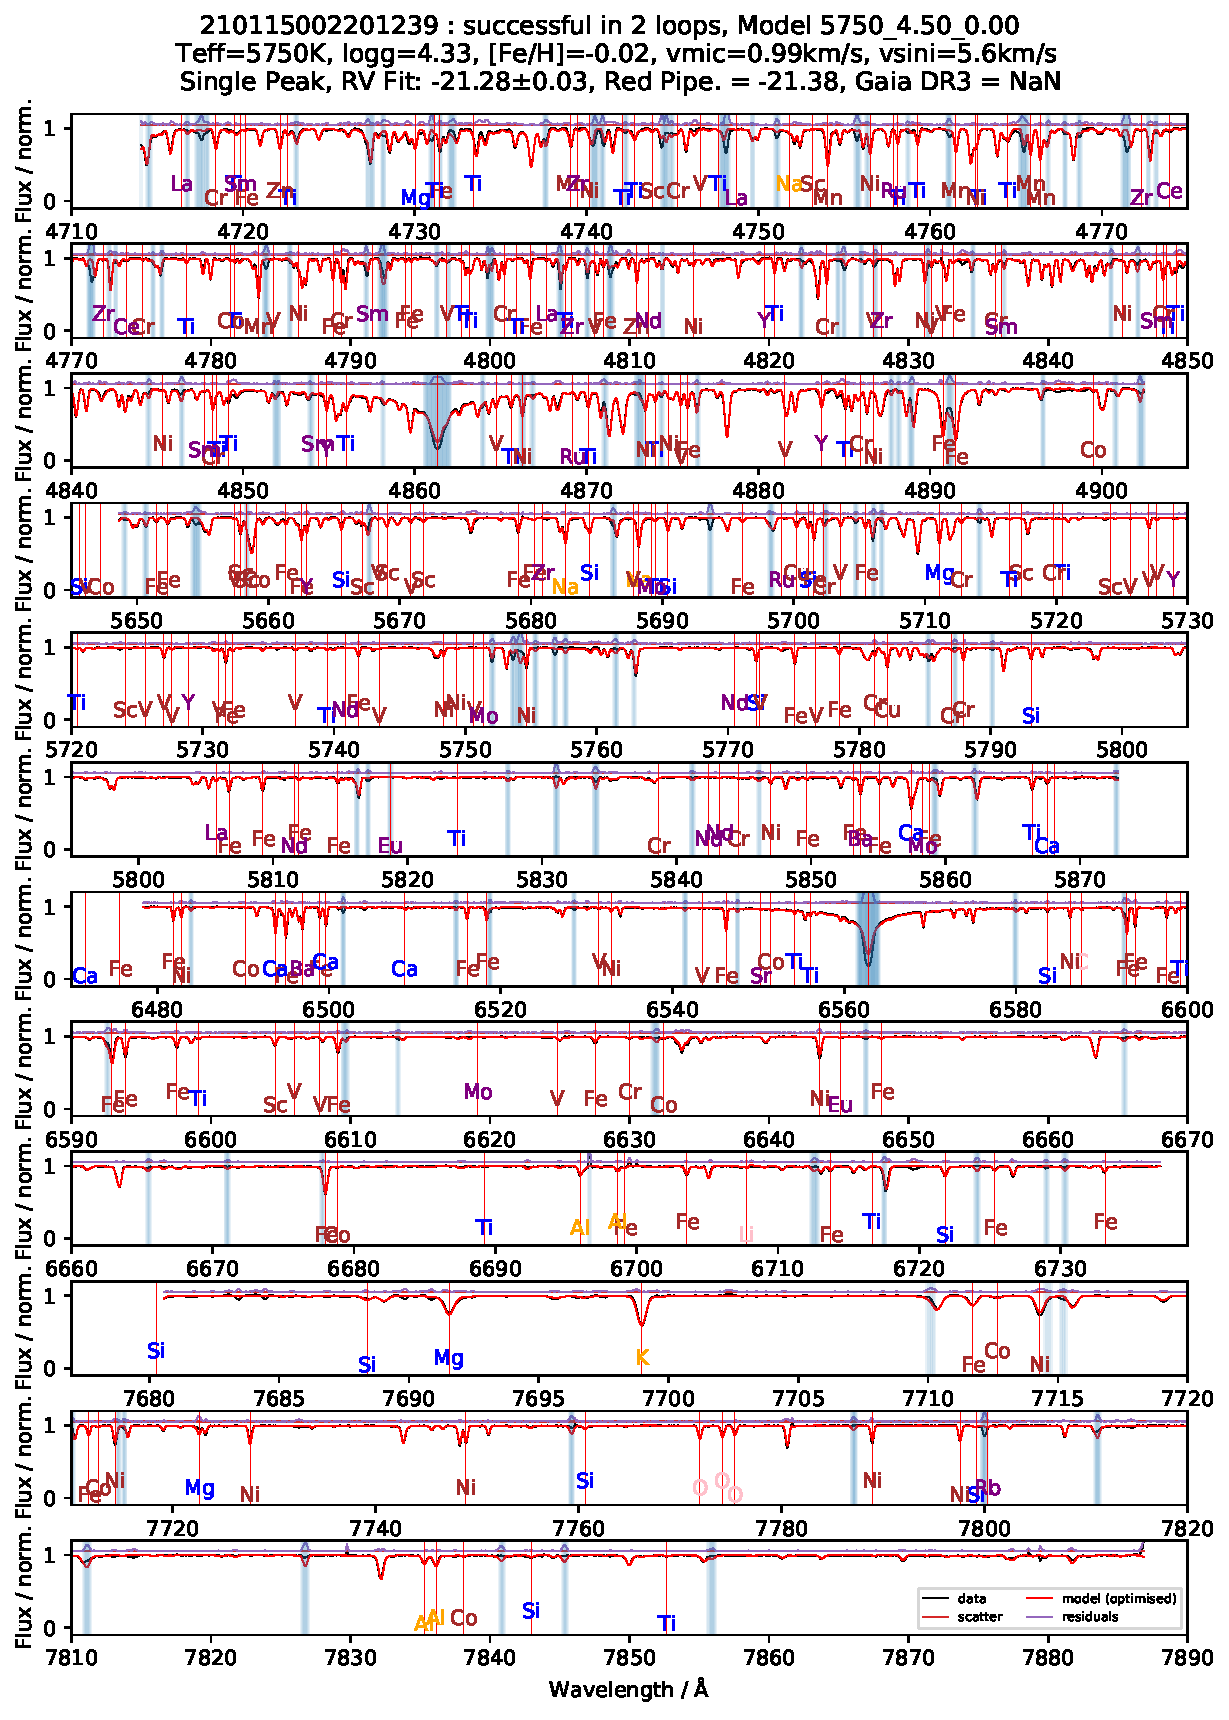
\includegraphics[width=0.9\textwidth]{figures/210115002201239_single_fit_comparison.pdf}
\caption{\textbf{Comparison of the observed (black) and best-fit spectrum (red) for the 2dF-HERMES spectrum of the asteroid 4~Vesta.} Important element lines are annotated in each of the wavelength regions colored by their element group. Vertical areas indicate masked regions that were neglected for the label optimisation, most notably $\mathrm{H}_\beta$ at $4861\,\text{\AA}$ and $\mathrm{H}_\alpha$ at $6563\,\text{\AA}$. \SB{Maybe actually use OmegaCen star 140314005201392: cool, metal-poor, strong CNO features and a good spectrum to explain why continuum points may not always work for a pipeline. See Sec.~\ref{sec:data_products_for_each_spectrum}}} \label{fig:210115002201239_single_fit_comparison}
\end{figure*}

\newpage
%%%%%%%%%%%%%%%%%%%%%%%%%%%%%%%%%%%%%%%%%%%%%%%%%%%%%%%%%%%%%%%%%%%%%%%%%
\section{CONCLUSIONS}
\label{sec:conclusion}
%%%%%%%%%%%%%%%%%%%%%%%%%%%%%%%%%%%%%%%%%%%%%%%%%%%%%%%%%%%%%%%%%%%%%%%%%

%%%%%%%%%%%%%%%%%%%%%%%%%%%%%%%%%%%%%%%%%%%%%%%%%%
\section*{Acknowledgements}
%%%%%%%%%%%%%%%%%%%%%%%%%%%%%%%%%%%%%%%%%%%%%%%%%%

We acknowledge the traditional owners of the land on which the AAT and ANU stand, the Gamilaraay, the Ngunnawal and Ngambri people. We pay our respects to elders past, present, and emerging and are proud to continue their tradition of surveying the night sky in the Southern hemisphere.
This work was supported by the Australian Research Council Centre of Excellence for All Sky Astrophysics in 3 Dimensions (ASTRO 3D), through project number CE170100013.

\section*{Facilities}

\textbf{AAT with 2df-HERMES at Siding Spring Observatory:}
AAT observations for this data relerase were performed under programs {2013B/13}, {2014A/25}, {2015A/3}, {2015A/19}, {2015B/1}, {2015B/19}, {2016A/22}, {2016B/10}, {2016B/12}, {2017A/14}, {2017A/18}, {2017B/16}, {2018A/18}, {2018B/15}, {2019A/1}, {2019A/15}, and {2020/B23}. This paper includes data that has been provided by AAO Data Central (datacentral.aao.gov.au).
\textbf{\Gaia: } This work has made use of data from the European Space Agency (ESA) mission \Gaia (\url{http://www.cosmos.esa.int/gaia}), processed by the \Gaia Data Processing and Analysis Consortium (DPAC, \url{http://www.cosmos.esa.int/web/gaia/dpac/consortium}). Funding for the DPAC has been provided by national institutions, in particular the institutions participating in the \Gaia Multilateral Agreement. 
\textbf{Other facilities:} This publication makes use of data products from the Two Micron All Sky Survey \citep{Skrutskie2006} and the CDS VizieR catalogue access tool \citep{Vizier2000}.

\section*{Software}

The research for this publication was coded in \textsc{python} (version 3.7.4) and included its packages
\textsc{astropy} \citep[v. 3.2.2;][]{Robitaille2013,PriceWhelan2018},
\textsc{astroquery} \citep[v. 0.4;][]{Ginsburg2019},
\textsc{corner} \citep[v. 2.0.1;][]{corner},
\textsc{galpy} \citep[version 1.6.0;][]{Bovy2015},
\textsc{IPython} \citep[v. 7.8.0;][]{ipython},
\textsc{matplotlib} \citep[v. 3.1.3;][]{matplotlib},
\textsc{NumPy} \citep[v. 1.17.2;][]{numpy},
\textsc{scipy} \citep[version 1.3.1;][]{scipy},
\textsc{sklearn} \citep[v. 0.21.3;][]{scikit-learn},
\textsc{statsmodels} (v. 0.10.1),
\textsc{xdgmm} (v. 1.1).
We further made use of \textsc{topcat} \citep[version 4.7;][]{Taylor2005};


% \begin{table*}
% \begin{threeparttable}
% \caption{Identified backscatter from objects in orbit and their properties}\label{satdet}
% \begin{tabular}{ c c c c c c } \toprule
% Satellite\tnote{a}   &NORAD           &Start      &End               &Mean intensity         &RCS\tnote{b}            \\
% name        &ID \#           &time (UT)       &time (UT)             & (Jy/beam)      &($m^{2}$)        \\ \midrule
% BGUSAT      & 41999 &2020-01-31 14:40:09.9  &2020-01-31 14:43:11.9  &1060  &$<$0.1       \\ 
% ISS (ZARYA) & 25544 &2020-01-31 17:17:41.9  &2020-01-31 17:19:00.9  &440  & $>$1.0      \\ 
% MAX VALIER SAT& 42778 &2020-02-03 01:18:16.9  &2020-02-03 01:20:09.9  &650  &0.1 $-$ 1.0       \\
% ISS (ZARYA) &22554 &2020-02-03 01:31:07.9  &2020-02-03 01:33:14.9  &930  &$>$1.0         \\ 
% FLOCK 3P 71 & 42024 &2020-02-01 14:16:22.9& 2020-02-01 14:18:05.9  &330  &$<$0.1       \\ 
% ISS (ZARYA) & 25544 &2020-02-02 02:18:17.9  &2020-02-02 02:20:16.9  &740  &$>$1.0 \\  
% BGUSAT      & 41999 &2020-02-02 02:18:17.9  &2020-02-02 02:20:16.9  &1010  &$<$0.1 \\ \bottomrule
% \end{tabular}
% \begin{tablenotes}
% \item[a] TLE information for predicted trajectories from space-track.org for the epoch of observation: 2020-02-01
% \item[b] Radar Cross Section (RCS) is categorised by space-track.org as: small ($<$0.1); medium (0.1 $<$ RCS $<$ 1.0); and large ($>$1.0)
% \end{tablenotes}
% \end{threeparttable}
% \end{table*}


\bibliography{bib}

\appendix

\section{Initial parameters}

\begin{figure*}[!ht]
 \centering
 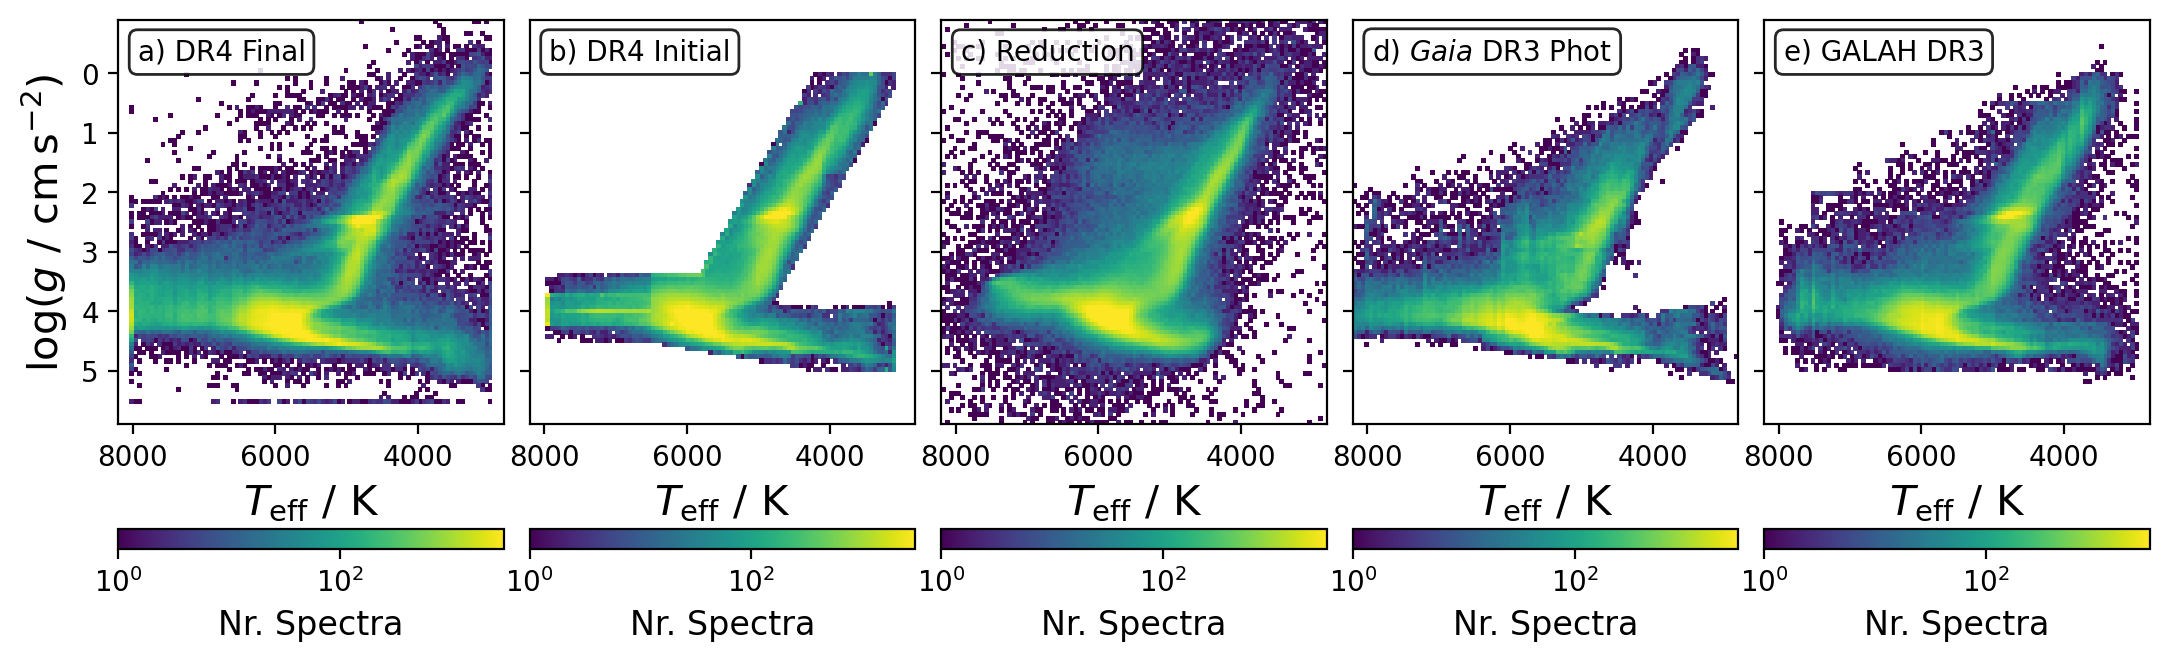
\includegraphics[width=\textwidth]{figures/initial_teff_logg.png}
 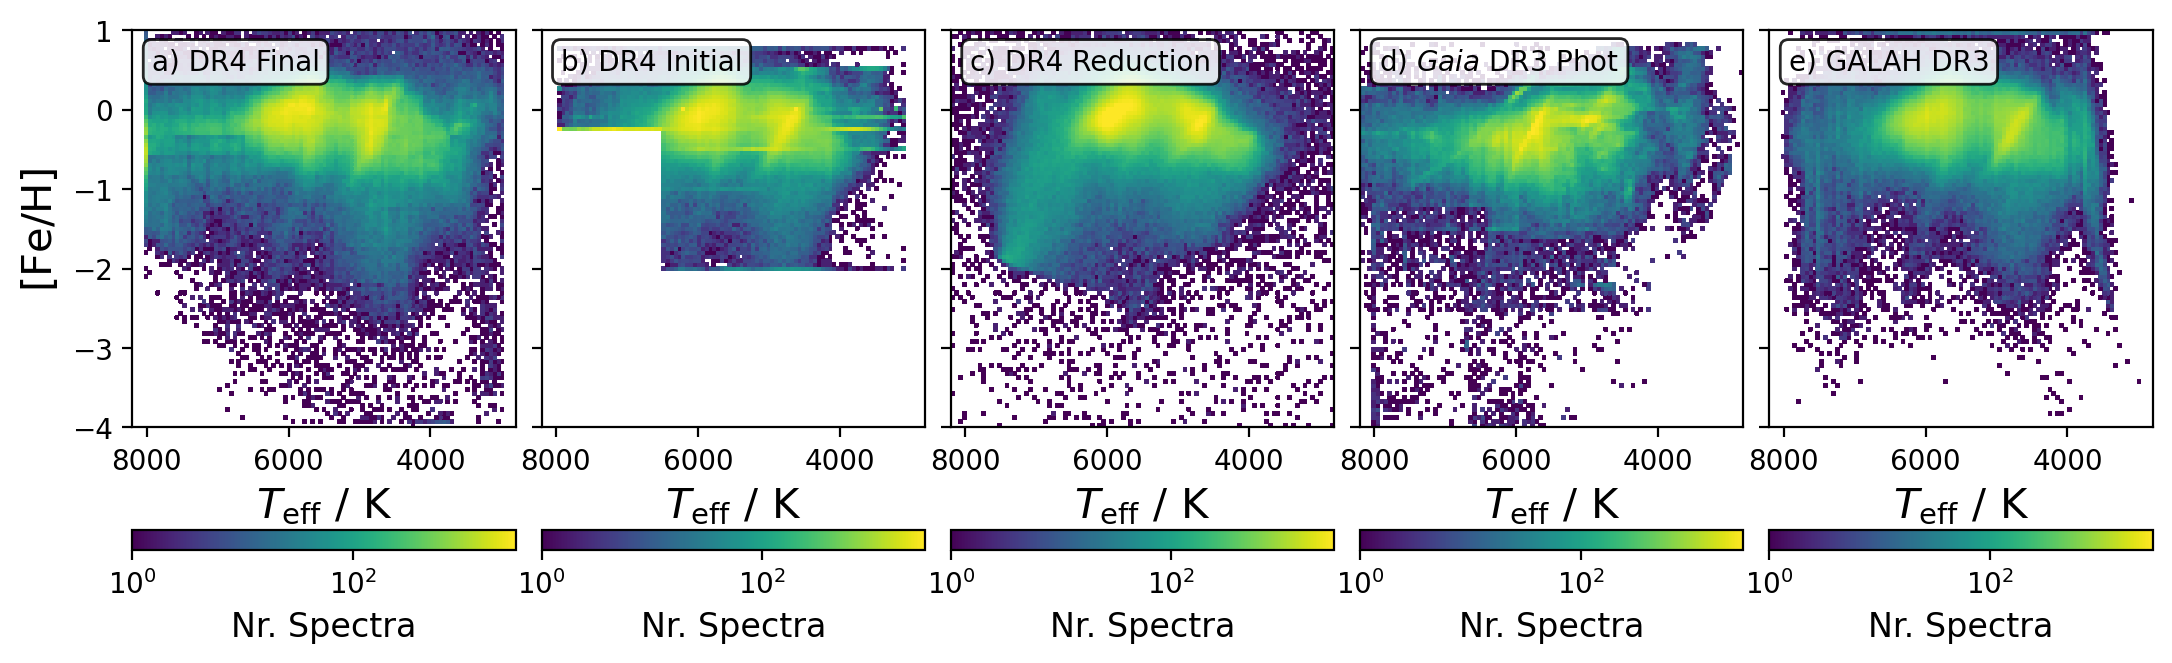
\includegraphics[width=\textwidth]{figures/initial_teff_fe_h.png}
 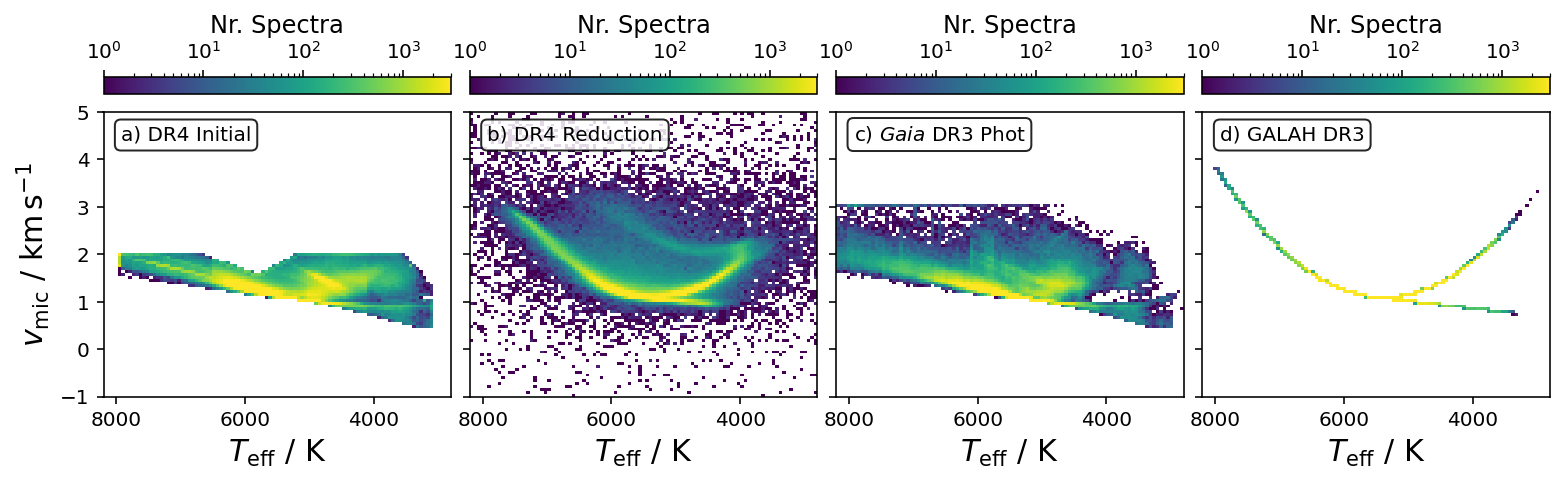
\includegraphics[width=\textwidth]{figures/initial_teff_vmic.png}
 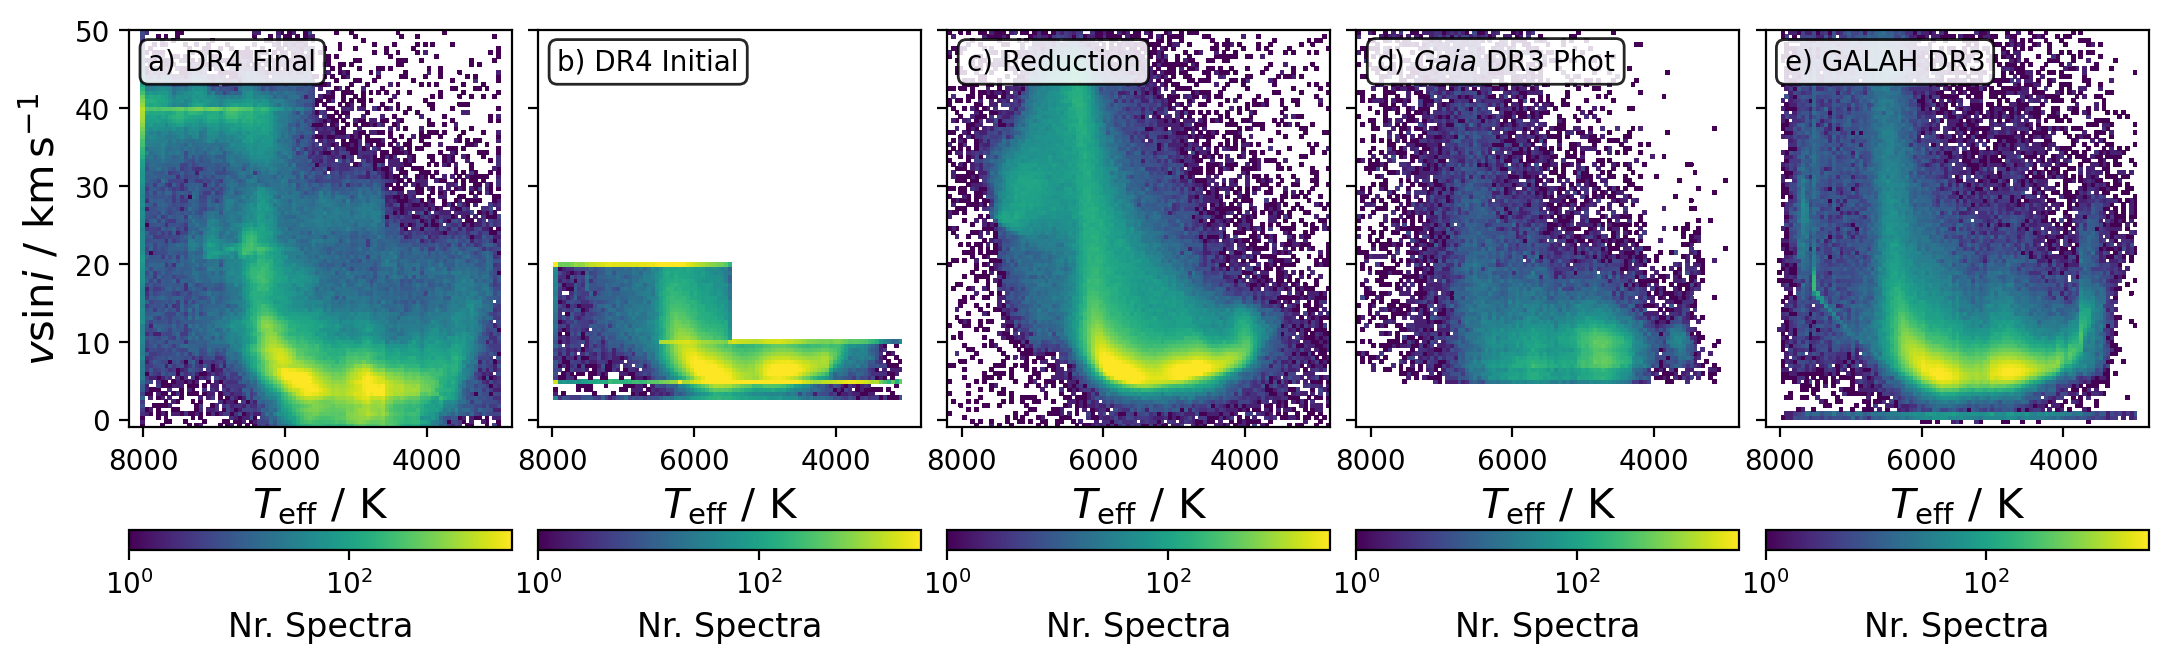
\includegraphics[width=\textwidth]{figures/initial_teff_vsini.png} \caption{\textbf{Comparison of initial parameters used for GALAH DR4 (first column) with the GALAH DR4 reduction pipeline (second column), \Gaia DR3 (third column with \vmic based on the adjusted formula from \citet{DutraFerreira2016}), and GALAH DR3 (fourth column).}} \label{fig:initial_parameters}
\end{figure*}


\end{document}
